\documentclass[aspectratio=169]{beamer}
%\usetheme{Simple}

\usepackage{listings}
%\usepackage{lmodern}
 \setbeamercovered{transparent}

 \usetheme[width=4\baselineskip,hideothersubsections]{Berkeley}

 \setbeamerfont{section in sidebar}{size=\scriptsize}
 \setbeamerfont{subsection in sidebar}{size=\tiny}

 \usepackage{multirow}


%% tikz stuff
\usepackage{tikz}
\usetikzlibrary{external}

\usetikzlibrary{shapes}
\usetikzlibrary{fit}

\newcounter{a}
\newcounter{b}
\usepackage{etoolbox} %for if empty functionality
\usepackage{ifthen}
\usepackage{leftidx}


%%equation stuff
\usepackage{braket}
\usepackage{amsmath} % Mathematical symbols
\usepackage{amssymb} % Symbols
\usepackage{amsfonts}
\usepackage{mathtools}
\usepackage{physics} %thing s.a. \Tr 


%%plot stuff
\usepackage{subcaption} % Subfigure environment 
\usepackage{caption}% Captions onder figuur gecentreerd
\usepackage{float}
\usepackage{graphicx}

%break long urls at a - and not only at . or /
\usepackage{url}
% \def\UrlBreaks{\do\/\do-}
% \usepackage{breakurl}
\usepackage{hyperref}

%environments
\usepackage{verbatim}
\usepackage{fancyvrb} %inline verbatim
\usepackage{cleveref} 

\usepackage[acronym]{glossaries}
\usepackage[toc,page]{appendix}
%\usepackage{acronym}

%random
\usepackage{booktabs}
\usepackage{lipsum}
\usepackage{epigraph}
\usepackage{pdfpages}
\usepackage{todonotes}


\allowdisplaybreaks %break multiline equations


%----------------------------------------------------------------------------------------
%	TITLE PAGE
%----------------------------------------------------------------------------------------

% The title
\title[]{  Cluster Expansions of Thermal States using Tensor Networks  }

\author[] {David Devoogdt}
\institute[UGent] % Your institution may be shorthand to save space
{
    % Your institution for the title page
    Faculty of Engineering and Architecture \\
    Ghent University 
    \vskip 3pt
}
\date{\today} % Date, can be changed to a custom date


%\def\temp{#1}\ifx\temp\empty
%  <EMPTY>%
%\else
%  <NON EMPTY>%
%\fi

\newcommand{\combineTikz}[3]{
    \begin{tikzpicture}[baseline={0-0.5*height("$=$")}]
        \node (AA) at (0,0)  { #1   };
        \node (AB) at ( {#3} ,0)  {  #2  };
    \end{tikzpicture}
}

%\newcommand{\mpo}[6]  {\tikzexternalenable { \begin{tikzpicture}[baseline={0-0.5*height("$=$")}]
\newcommand{\mpo}[6]  { \begin{tikzpicture}[baseline={0-0.5*height("$=$")}]

        %\def \NNodes {#1}
        %\def \NodeName {#2}          
        %\def \NodeName {#2}          
        %\def \NodeName {#2}          
        %\def \NodeName {#2}          
        %\def \NodeName {#2}          
        %\def \NameUp   {#3} 
        %\def \NameUp   {#3} 
        %\def \NameUp   {#3} 
        %\def \NameUp   {#3} 
        %\def \NameUp   {#3} 
        %\def \NameDown  {#4}	
        %\def \NameDown  {#4}	
        %\def \NameDown  {#4}	
        %\def \NameDown  {#4}	
        %\def \NameDown  {#4}	

        \def \legLength {0.7}
        \def \radius {0.3}

        \pgfmathsetmacro{\step}{2*\radius+\legLength}
        \pgfmathsetmacro{\legpos}{\radius+\legLength}

        \pgfmathsetmacro{\Nmax}{#1-1}

        \foreach \N in {0,..., \Nmax }{
                \pgfmathsetmacro{\p}{\N*\step}

                % up and down labels
                \def\temp{#3}\ifx\temp\empty
                    \def \labelUp {}
                \else
                    \pgfmathsetmacro{\labelUp}{  {#3}[\N]  }
                \fi

                \def\tempp{#4}\ifx\tempp\empty
                    \def \labeldown {}
                \else
                    \pgfmathsetmacro{\labeldown}{  {#4}[\N]  }
                \fi

                \def\aab{#5}\ifx\aab\empty
                    \def \dotssite {0}
                \else
                    \pgfmathsetmacro{\dotssite}{  {#5}[\N]  }
                \fi

                \ifthenelse{\dotssite = 0}{

                    \def\aac{#6}\ifx\aac\empty
                        \def \nname {O}
                    \else
                        \pgfmathsetmacro{\nname}{  {#6}[\N]  }
                    \fi

                    \node[circle,draw, radius=\radius] (O\N) at (\p,0) {\nname};

                    \ifthenelse{ \equal{\labelUp}{-}  }{
                    }{
                        \node[] (Ou\N) at (\p, \legpos ) { \labelUp };
                        \draw (O\N) -- (Ou\N);
                    }

                    \ifthenelse{ \equal{\labeldown}{-}  }{
                    }{
                        \node[] (Od\N) at (\p,-\legpos) {\labeldown};
                        \draw (O\N) -- (Od\N);
                    }

                }{
                    \node[circle] (O\N) at (\p,0) { $\cdots$ };
                }

            }

        \ifthenelse{  #1  =1  }{}{
            \foreach \N in {1,...,\Nmax }{
                    \pgfmathsetmacro{\M}{\N-1}
                    \pgfmathsetmacro{\label}{ {#2}[\N]  }
                    %\pgfmathsetmacro{\label}{ 5}

                    \draw (O\M) --  node[above]  {\label} (O\N);
                }
        }

        \pgfmathsetmacro{\labelo}{ {#2}[0]}
        \pgfmathsetmacro{\labeli}{  {#2}[\Nmax+1]}

        \ifthenelse{ \equal{\labelo}{Tr}  }{

            \pgfmathsetmacro{\endpos}{\step*\Nmax+\radius}

            \draw plot [smooth ]  coordinates { (-\radius,0)    (-\radius, -0.45 )  (\endpos, -0.45)   (O\Nmax)   } ;
        }{
            \ifthenelse{ \equal{\labelo}{-}  }{
            }{
                \pgfmathsetmacro{\endpos}{\step*\Nmax+\legpos}

                \node (N0) at (-\legpos,0) {};
                \node (Ne) at (\endpos,0) {};

                \draw (N0) -- node[above] {\labelo} (O0);

                \draw (Ne) -- node[above] {\labeli}  (O\Nmax);
            }
        }
        %\draw (O0) --  node[above] {1} (O1);
        %\end{tikzpicture}} \tikzexternaldisable}
    \end{tikzpicture}}

%\newcommand{\expH}[5]{\tikzexternalenable { \begin{tikzpicture}[baseline={0-0.5*height("$=$")}]
\newcommand{\expH}[5]{\begin{tikzpicture}[baseline={0-0.5*height("$=$")}]
        \def \NNodes {#1};

        \def\aaa{#2}\ifx\aaa\empty
            \def \text { $e^{-\beta \hat{H}_{\NNodes} }$ }
        \else
            \def \text {#2}
        \fi

        \pgfmathwidth{ "\text" }
        \def \textwidth { \pgfmathresult }

        %\pgfmathsetmacro{\text}{width(\text)}

        \def \legLength {0.6}
        \def \radius {0.3} %fix to fit text inside for size 1
        \def \boxHeight {0.4};

        \pgfmathsetmacro{\step}{2*\radius+\legLength}
        \pgfmathsetmacro{\legpos}{\radius+\legLength}
        \pgfmathsetmacro{\dotpos}{\boxHeight+\legLength/2}

        \pgfmathsetmacro{\Nmax}{\NNodes -1}

        \pgfmathsetmacro{\boxsize}{ max ( \textwidth/1cm , \step*\Nmax )   + \radius}

        %\pgfmathsetmacro{\boxsize}{ 5  )}
        %\pgfmathsetlength{\boxsize}{ max( \textwidth,  \boxsize1  )}

        %            \ifthenelse{#1=1}{
        %                \def \left {-0.6}
        %                \def \right {0.6}
        %            }{
        \def \left {-\radius}
        \def \right {\boxsize}
        %            }

        \draw (\left,- \boxHeight ) rectangle (\right, \boxHeight ) [add reference =H] ;

        \node  at (H center) { \text };

        \foreach \N in {0,..., \Nmax }{
                \pgfmathsetmacro{\p}{\N*\step}

                % up and down labels
                \def\temp{#3}\ifx\temp\empty
                    \def \labelUp {}
                \else
                    \pgfmathsetmacro{\labelUp}{  {#3}[\N]  }
                \fi

                \def\tempp{#4}\ifx\tempp\empty
                    \def \labeldown {}
                \else
                    \pgfmathsetmacro{\labeldown}{  {#4}[\N]  }
                \fi

                \node[] (O\N) at (\p,0) {};

                \ifthenelse{ \equal{\labelUp}{...}  }{
                    \node[] (Ou\N) at (\p, \dotpos ) {\labelUp};
                }{
                    \ifthenelse{ \equal{\labelUp}{-}  }{

                    }{
                        \node[] (Ou\N) at (\p, \legpos ) {\labelUp};
                        \draw (Ou\N) --  (Ou\N  |- H north);
                    }
                }

                \ifthenelse{ \equal{\labeldown}{...}  }{
                    \node[] (Od\N) at (\p,-\dotpos ) {\labeldown};
                }{
                    \ifthenelse{ \equal{\labeldown}{-}  }{

                    }{
                        \node[] (Od\N) at (\p,-\legpos) {\labeldown};
                        \draw (Od\N) --  (Od\N  |- H south);
                    }
                }
            }

        \def\tempt{#5}\ifx\tempt\empty

        \else
            \pgfmathsetmacro{\labelo}{ {#5}[0] }
            \pgfmathsetmacro{\labeli}{  {#5}[1] }

            \pgfmathsetmacro{\leftleg}{  \left - \legLength }
            \pgfmathsetmacro{\rightleg}{  \right + \legLength }

            \node (N0) at (\leftleg,0) {\labelo};
            \draw (N0) -- ( N0  -| H west);

            \node (Ne) at (\rightleg,0) {\labeli};
            \draw (Ne) --  ( Ne  -| H east);
        \fi

        %        \end{tikzpicture}} \tikzexternaldisable }
    \end{tikzpicture} }

%\newcommand{\mpob}[6]  {\tikzexternalenable { \begin{tikzpicture}[baseline={0-0.5*height("$=$")},scale=0.8]
\newcommand{\mpob}[6]  {\begin{tikzpicture}[baseline={0-0.5*height("$=$")},scale=0.8]

        %\def \NNodes {#1}
        %\def \NodeName {#2}          
        %\def \NodeName {#2}          
        %\def \NodeName {#2}          
        %\def \NodeName {#2}          
        %\def \NodeName {#2}          
        %\def \NameUp   {#3} 
        %\def \NameUp   {#3} 
        %\def \NameUp   {#3} 
        %\def \NameUp   {#3} 
        %\def \NameUp   {#3} 
        %\def \NameDown  {#4}	
        %\def \NameDown  {#4}	
        %\def \NameDown  {#4}	
        %\def \NameDown  {#4}	
        %\def \NameDown  {#4}	

        \def \legLength {1.0}
        \def \radius {0.1}

        \pgfmathsetmacro{\step}{2*\radius+\legLength}
        \pgfmathsetmacro{\legpos}{\radius+\legLength}

        \pgfmathsetmacro{\Nmax}{#1-1}

        \foreach \N in {0,..., \Nmax }{
                \pgfmathsetmacro{\p}{\N*\step}

                % up and down labels
                \def\temp{#3}\ifx\temp\empty
                    \def \labelUp {}
                \else
                    \pgfmathsetmacro{\labelUp}{  {#3}[\N]  }
                \fi

                \def\tempp{#4}\ifx\tempp\empty
                    \def \labeldown {}
                \else
                    \pgfmathsetmacro{\labeldown}{  {#4}[\N]  }
                \fi

                \def\aab{#5}\ifx\aab\empty
                    \def \dotssite {0}
                \else
                    \pgfmathsetmacro{\dotssite}{  {#5}[\N]  }
                \fi

                \def\aac{#6}\ifx\aac\empty
                    \def \nname { "O" }
                \else
                    \pgfmathsetmacro{\nname}{  {#6}[\N]  }
                \fi

                %\node[] (O\N) at (\p,0) {\nname};
                \node[circle,draw, radius=\radius] (O\N) at (\p,0) {\nname};

            }

        \ifthenelse{  #1  =1  }{}{
            \foreach \N in {1,...,\Nmax }{
                    \pgfmathsetmacro{\M}{\N-1}
                    \pgfmathsetmacro{\label}{ {#2}[\N]  }
                    %\pgfmathsetmacro{\label}{ 5}

                    \draw (O\M) --  node[above]  {\label} (O\N);
                }
        }

        % \pgfmathsetmacro{\labelo}{ {#2}[0]}
        % \pgfmathsetmacro{\labeli}{  {#2}[\Nmax+1]}

        % \node (N0) at (-\legpos,0) {};
        % \draw (N0) -- node[above] {\labelo} (O0);

        % \pgfmathsetmacro{\endpos}{\step*\Nmax+\legpos}

        % \node (Ne) at (\endpos,0) {};
        % \draw (Ne) -- node[above] {\labeli} (O\Nmax);

        %\draw (O0) --  node[above] {1} (O1);

        % \end{tikzpicture}} \tikzexternaldisable}

    \end{tikzpicture}}

% \newcommand{\pepob}[5]  { \tikzexternalenable {\begin{tikzpicture}[baseline={0-0.5*height("$=$")},scale=0.8]
% \newcommand{\pepob}[5]  { \begin{tikzpicture}[baseline={0-0.5*height("$=$")},scale=1,
\newcommand{\pepob}[5]  { \begin{tikzpicture}[
            baseline={([yshift= -2ex ]current bounding box.north)},
            %baseline={0-0.5*height("$=$")},
            scale=1,
            Al/.style = {regular polygon, regular polygon sides=3,
                    draw, fill=white, text width=0.1,
                    inner sep=1mm, outer sep=0mm,
                    shape border rotate=-90},
            Ar/.style = {regular polygon, regular polygon sides=3,
                    draw, fill=white, text width=0.1,
                    inner sep=1mm, outer sep=0mm,
                    shape border rotate=90},
            Acc/.style = {diamond, draw, inner sep=1mm},
            Ac/.style = {rectangle, draw, inner sep=2mm}]

        %\pgfmathsetmacro{\llegLength}{ 0.3 }

        \def \legLength { 0.8}
        \def \radius {0.1}

        %\pgfmathtruncatemacro{\llegLength} { 0.8 }
        %\pgfmathtruncatemacro{\radius} { 0.1 }

        %\pgfmathtruncatemacro{\legLength}{2* \llegLength}
        %\pgfmathtruncatemacro{\lstep}{\radius+ \llegLength}
        %\pgfmathtruncatemacro{\step}{2*\lstep}
        \pgfmathsetmacro{\step}{2*\radius+ \legLength}

        \pgfmathsetmacro{\legpos}{\radius+\legLength}

        \pgfmathsetmacro{\Nmax}{#1-1}
        \pgfmathsetmacro{\Mmax}{#2-1}

        % define positions of different O's

        \setcounter{a}{0}
        %\setcounter{a}{0}

        \foreach \N in {0,..., \Nmax }{

                %\pgfmathtruncatemacro{\a}{\thea}

                \pgfmathsetmacro{\p}{  (\N + \thea) *\step   }
                %\setcounter{b}{0}

                \foreach \M in {0,..., \Mmax }{

                        %\pgfmathsetmacro{\p}{ \pp + \theb *\step   }

                        \pgfmathsetmacro{\k}{   \M   *\step  }

                        \pgfmathtruncatemacro{\s}{\M*(\Nmax+1)+\N   }

                        \pgfmathsetmacro{\nname}{ ""  }

                        \def\aab{#5}\ifx\aab\empty
                            \def \so {0}
                        \else
                            \pgfmathsetmacro{\so}{  {#5}[\s]  }
                        \fi

                        \ifthenelse{\so = 0}{
                            \node[circle,draw, radius=\radius] (O\s) at (\p,\k) {\nname};
                        }

                        \ifthenelse{\so = 2}{
                            \node[draw, Al] (O\s) at (\p,\k) {\nname};
                        }

                        \ifthenelse{\so = 3}{
                            \node[draw, Ar] (O\s) at (\p,\k) {\nname};
                        }

                        \ifthenelse{\so = 4}{
                            \node[draw= none, inner sep=0, outer sep=0 , minimum size=0pt] (O\s) at (\p,\k) {\nname};
                        }

                        \ifthenelse{\so = 6}{
                            \node[draw, Acc] (O\s) at (\p,\k) {\nname};
                        }

                        \ifthenelse{\so = 7}{
                            \node[draw, Ac] (O\s) at (\p,\k) {\nname};
                        }

                        %Gl environment
                        \ifthenelse{\so = 5}{

                            \pgfmathsetmacro{\recl}{  \p + \step - 3*\radius  }
                            \pgfmathsetmacro{\recr}{  \p + \step + 3*\radius  }

                            \pgfmathsetmacro{\recu}{  \k + 2*\radius }
                            \pgfmathsetmacro{\recd}{  \k - \step -2*\radius  }

                            % \pgfmathsetmacro{\recl}{  \p  +\step   }
                            % \pgfmathsetmacro{\mw}{ 2*\radius }
                            % \pgfmathsetmacro{\mh}{ \step  }

                            % \pgfmathsetmacro{\recu}{  \k - \step /2 }

                            % \node[rectangle,
                            %     draw,
                            %     minimum height= 1,
                            %     anchor=center  ] (O\s) at (\recl,\recu) {Gl};

                            \draw  (\recl,\recu) rectangle node[  ] (O\s)  {Gl}   (\recr,\recd)     ;

                            %\draw node[fill, minimum width= 1  ,minimum height= 1 ] (O\s) at (\recl,\recu) {Gl};
                            \stepcounter{a}
                        }

                        \ifthenelse{\so = 8}{

                            \node[draw, Ar] (O\s) at (\p,\k) {\nname};

                            \pgfmathtruncatemacro{\t}{\M*(\Nmax+1)+\N +1  }

                            \pgfmathsetmacro{\recl}{  \p +\step  - 3*\radius  }
                            \pgfmathsetmacro{\recr}{  \p + \step+  3*\radius  }

                            \pgfmathsetmacro{\recu}{  \k + 2*\radius }
                            \pgfmathsetmacro{\recd}{  \k - \step -2*\radius  }

                            \draw  (\recl,\recu) rectangle node (O\t)  {Gr}   (\recr,\recd)     ;

                            \draw  (O\s) -- (   O\t.west   |-  O\s  ) ;
                            \stepcounter{a}
                        }

                        \ifthenelse{\so = 9}{

                            \node[draw, Ac] (O\s) at (\p,\k) {\nname};

                            \pgfmathtruncatemacro{\t}{\M*(\Nmax+1)+\N +1  }

                            \pgfmathsetmacro{\recl}{  \p +\step  - 3*\radius  }
                            \pgfmathsetmacro{\recr}{  \p + \step+  3*\radius  }

                            \pgfmathsetmacro{\recu}{  \k + 2*\radius }
                            \pgfmathsetmacro{\recd}{  \k - \step -2*\radius  }

                            \draw  (\recl,\recu) rectangle node (O\t)  {Gr}   (\recr,\recd)     ;

                            \draw  (O\s) -- (   O\t.west   |-  O\s  ) ;
                            \stepcounter{a}
                        }

                        \ifthenelse{\so = 10}{

                            \node[draw = none] (O\s) at (\p,\k) {\nname};

                            \pgfmathtruncatemacro{\t}{\M*(\Nmax+1)+\N +1  }

                            \pgfmathsetmacro{\recl}{  \p +\step  - 3*\radius  }
                            \pgfmathsetmacro{\recr}{  \p + \step+  3*\radius  }

                            \pgfmathsetmacro{\recu}{  \k + 2*\radius }
                            \pgfmathsetmacro{\recd}{  \k - \step -2*\radius  }

                            \draw  (\recl,\recu) rectangle node (O\t)  {Gr}   (\recr,\recd)     ;

                            \draw  (O\s) -- (   O\t.west   |-  O\s  ) ;
                            \stepcounter{a}
                        }

                        \ifthenelse{\so = 11}{

                            \node[draw , Acc] (O\s) at (\p,\k) {\nname};

                            \pgfmathtruncatemacro{\t}{\M*(\Nmax+1)+\N +1  }

                            \pgfmathsetmacro{\recl}{  \p +\step  - 3*\radius  }
                            \pgfmathsetmacro{\recr}{  \p + \step+  3*\radius  }

                            \pgfmathsetmacro{\recu}{  \k + 2*\radius }
                            \pgfmathsetmacro{\recd}{  \k - \step -2*\radius  }

                            \draw  (\recl,\recu) rectangle node (O\t)  {Gr}   (\recr,\recd)     ;

                            \draw  (O\s) -- (   O\t.west   |-  O\s  ) ;
                            \stepcounter{a}
                        }

                        \ifthenelse{\so = 12}{

                            \node[circle,draw, radius=\radius] (O\s) at (\p,\k) {\nname};

                            \pgfmathsetmacro{\pp}{   \p+\legLength/2 }
                            \pgfmathsetmacro{\pm}{   \p-\legLength/2  }

                            \pgfmathsetmacro{\kp}{   \k+\legLength/2  }
                            \pgfmathsetmacro{\km}{   \k-\legLength/2  }

                            \node (Op\s) at (\pp,\kp) {i};
                            \node (Om\s) at (\pm,\km) {j};

                            \draw (O\s.center)  --  (Op\s);
                            \draw  (Om\s) --  (O\s);
                        }

                        \ifthenelse{\so = 13}{

                            \node[draw= none] (O\s) at (\p,\k) { ... };
                        }

                        \ifthenelse{\so = 14}{

                            \node[circle,draw, radius=\radius] (O\s) at (\p,\k) {\nname};

                            \pgfmathsetmacro{\pp}{   \p+\legLength/2 }
                            \pgfmathsetmacro{\pm}{   \p-\legLength/2  }

                            \pgfmathsetmacro{\kp}{   \k+\legLength/2  }
                            \pgfmathsetmacro{\km}{   \k-\legLength/2  }

                            \node (Op\s) at (\pp,\kp) {};
                            \node (Om\s) at (\pm,\km) {};

                            \draw (O\s.center)  --  (Op\s);
                            \draw  (Om\s) --  (O\s);
                        }

                        \ifthenelse{\so = 15}{

                            \node[circle,draw, radius=\radius] (O\s) at (\p,\k) {\nname};

                            \pgfmathsetmacro{\pp}{   \p+\legLength/2 }

                            \pgfmathsetmacro{\kp}{   \k+\legLength/2  }

                            \node (Op\s) at (\pp,\kp) {};

                            \draw (O\s.center)  --  (Op\s);
                        }

                        \ifthenelse{\so = 16}{
                            \node[draw, Ac] (O\s) at (\p,\k) {B};
                        }

                        \ifthenelse{\so = 17}{
                            \node[circle,draw=none, radius=\radius] (O\s) at (\p,\k) {\nname};
                        }

                        \ifthenelse{\so = 18}{

                            \node[circle,draw=none, radius=\radius] (O\s) at (\p,\k) {\nname};

                            \pgfmathtruncatemacro{\t}{\M*(\Nmax+1)+\N +1  }

                            \pgfmathsetmacro{\recl}{  \p +\step  - 3*\radius  }
                            \pgfmathsetmacro{\recr}{  \p + \step+  3*\radius  }

                            \pgfmathsetmacro{\recu}{  \k + 2*\radius }
                            \pgfmathsetmacro{\recd}{  \k - \step -2*\radius  }

                            \draw  (\recl,\recu) rectangle node (O\t)  {Gr}   (\recr,\recd)     ;

                            \draw  (O\s) -- (   O\t.west   |-  O\s  ) ;
                            \stepcounter{a}
                        }

                        \ifthenelse{\so = 22}{
                            \node[draw,line width=0.6mm  ,Al] (O\s) at (\p,\k) {};
                        }

                        \ifthenelse{\so = 23}{
                            \node[draw,line width=0.6mm  ,Ar] (O\s) at (\p,\k) {};
                        }

                        \ifthenelse{\so = 25}{
                            \node[draw,line width=0.6mm ,Ac] (O\s) at (\p,\k) {};
                        }

                        \ifthenelse{\so = 24}{
                            \node[draw, Ac] (O\s) at (\p,\k) {Fl};
                        }

                        \ifthenelse{\so = 26}{
                            \node[draw, Ac] (O\s) at (\p,\k) {Fr};
                        }

                    }
            }

        %connect nodes horizontally with correct name
        \foreach \M in {0,..., \Mmax }{
                \foreach \N in {1,...,\Nmax}{

                        \pgfmathtruncatemacro{\s}{\M*(\Nmax+1)+\N   }

                        \pgfmathtruncatemacro{\t}{\M*(\Nmax+1)+\N  -1 }

                        \pgfmathtruncatemacro{\l}{\M*(\Nmax)+\N -1 }

                        %\pgfmathsetmacro{\label}{ {#2}[\N]  }
                        %\pgfmathsetmacro{\label}{ \l }
                        \pgfmathsetmacro{\label}{ {#3}[\l]  }

                        \def\aab{#5}\ifx\aab\empty
                            \def \so {0}
                        \else
                            \pgfmathsetmacro{\so}{  {#5}[\s]  }
                        \fi

                        \def\aab{#5}\ifx\aab\empty
                            \def \to {0}
                        \else
                            \pgfmathsetmacro{\to}{  {#5}[\t]  }
                        \fi

                        \ifthenelse{ \equal{\label}{Gl}  }{

                            \pgfmathtruncatemacro{\ogl}{ (\M+1)*(\Nmax+1)+\N -1 }

                            \draw (O\ogl.east   |- O\s  )  --  (O\s);

                            \draw (O\t)  --  ( O\ogl.west    |-  O\t  );

                        }{

                            \ifthenelse{ \equal{\label}{Gr}  }{

                                \pgfmathtruncatemacro{\ogl}{ (\M+1)*(\Nmax+1)+\N  }

                                \draw (O\t)  --  ( O\ogl.west    |-  O\t  );

                                \draw (O\ogl.east   |- O\s  )  --  (O\s);

                            }{

                                \ifthenelse{ \NOT  \so = 1  }{
                                    \ifthenelse{ \NOT  \to = 1}{
                                        \ifthenelse{ \equal{\label}{-} }{

                                        }
                                        {

                                            \draw ( O\t.east |- O\s )  --  node[above]  {\label} (O\s);
                                        }
                                    }
                                }
                            }

                        }

                    }
            }

        %connect nodes vertically with correct name
        \foreach \N in {0,...,\Nmax }{
                \foreach \M in {1,..., \Mmax }{

                        \pgfmathtruncatemacro{\s}{\M*(\Nmax+1)+\N   }

                        \pgfmathtruncatemacro{\t}{ (\M-1)*(\Nmax+1)+\N  }

                        \pgfmathtruncatemacro{\l}{\N*\Mmax+\M  -1 }

                        %\pgfmathsetmacro{\label}{ {#4}[\l]  }
                        \pgfmathsetmacro{\label}{ {#4}[\l]  }

                        \def\aab{#5}\ifx\aab\empty
                            \def \so {0}
                        \else
                            \pgfmathsetmacro{\so}{  {#5}[\s]  }
                        \fi

                        \def\aab{#5}\ifx\aab\empty
                            \def \to {0}
                        \else
                            \pgfmathsetmacro{\to}{  {#5}[\t]  }
                        \fi

                        % \pgfmathtruncatemacro{\st}{ \so+\to  }

                        % \ifthenelse{\st = 0}{
                        %     \draw (O\t) --  node[left]  {\label} (O\s);
                        % }

                        \ifthenelse{ \( \NOT  \so = 1 \) \AND \( \NOT  \so = 5 \) }{
                            \ifthenelse{ \NOT  \to = 1}{
                                \ifthenelse{ \equal{\label}{-} }{

                                }
                                {
                                    \draw (O\t) --  node[left]  {\label} (O\s);
                                }
                            }
                        }

                    }
            }

        % \pgfmathsetmacro{\labelo}{ {#2}[0]}
        % \pgfmathsetmacro{\labeli}{  {#2}[\Nmax+1]}

        % \node (N0) at (-\legpos,0) {};
        % \draw (N0) -- node[above] {\labelo} (O0);

        % \pgfmathsetmacro{\endpos}{\step*\Nmax+\legpos}

        % \node (Ne) at (\endpos,0) {};
        % \draw (Ne) -- node[above] {\labeli} (O\Nmax);

        %\draw (O0) --  node[above] {1} (O1);

        % \pgfmathsetmacro{\s}{\Nmax*\step+0.5}
        % \pgfmathsetmacro{\t}{\Mmax*\step+0.5}

        % \draw[draw=none] (-0.5,-0.5) |- (\s,\t) |- cycle;

        %\end{tikzpicture}} \tikzexternaldisable}
    \end{tikzpicture}}


\tikzset{add reference/.style={insert path={%
                    coordinate [pos=0,xshift=-0.5\pgflinewidth,yshift=-0.5\pgflinewidth] (#1 south west)
                    coordinate [pos=1,xshift=0.5\pgflinewidth,yshift=0.5\pgflinewidth]   (#1 north east)
                    coordinate [pos=.5] (#1 center)
                    (#1 south west |- #1 north east)     coordinate (#1 north west)
                    (#1 center     |- #1 north east)     coordinate (#1 north)
                    (#1 center     |- #1 south west)     coordinate (#1 south)
                    (#1 south west -| #1 north east)     coordinate (#1 south east)
                    (#1 center     -| #1 south west)     coordinate (#1 west)
                    (#1 center     -| #1 north east)     coordinate (#1 east)
                }}}

\def \figa { \vcenter{\hbox{ \pepob{5}{3}{{
                        "","","","",
                        "","","","",
                        "","","",""}}{{
                        "","",
                        "","",
                        "","",
                        "","",
                        "",""}}{{
                        1,1,1,1,1,
                        1,0,0,0,1,
                        1,0,0,0,1}} } }}

\def \figb { \vcenter{\hbox{  \begin{tikzpicture}[baseline=0.5]

                \def \legLength { 0.8}
                \def \radius {0.1}

                \pgfmathsetmacro{\step}{2*\radius+ \legLength} % 1
                \pgfmathsetmacro{\legpos}{\radius+\legLength} %0.9

                \node[draw, circle,radius=\radius] (L0) at (-1,0) {};
                \node[draw, circle,radius=\radius] (L1) at (-1,1) {};

                \draw (-0.3,1.3) -- (0.3,1.3) -- (0.3,-0.3) -- (-0.3,-0.3) -- cycle;

                \node[draw, circle,radius=\radius] (R0) at (1,0) {};
                \node[draw, circle,radius=\radius] (R1) at (1,1) {};

                \draw (L0) --   (L1);
                \draw (R0) --   (R1);

                \draw (L0) --   (-0.3,0);
                \draw (L1) --   (-0.3,1);

                \draw (R0) --   (0.3,0);
                \draw (R1) --   (0.3,1);

                \node[draw=none] (C0) at (0,0.5) {X};
            \end{tikzpicture}}}}

\def \figc {\vcenter{\hbox{  \begin{tikzpicture}[baseline=0.5]

                \def \legLength { 0.8}
                \def \radius {0.1}

                \pgfmathsetmacro{\step}{2*\radius+ \legLength} % 1
                \pgfmathsetmacro{\legpos}{\radius+\legLength} %0.9

                \node[draw=none, circle,radius=\radius] (L0) at (-1,0) {};
                \node[draw=none, circle,radius=\radius] (L1) at (-1,1) {};

                \draw (-0.3,1.3) -- (0.3,1.3) -- (0.3,-0.3) -- (-0.3,-0.3) -- cycle;

                \node[draw=none, circle,radius=\radius] (R0) at (1,0) {};
                \node[draw=none, circle,radius=\radius] (R1) at (1,1) {};

                \draw (L0) --   (-0.3,0);
                \draw (L1) --   (-0.3,1);

                \draw (R0) --   (0.3,0);
                \draw (R1) --   (0.3,1);

                \node[draw=none] (C0) at (0,0.5) {X};
            \end{tikzpicture} }} }

\def \figd {\vcenter{\hbox{  \begin{tikzpicture}[baseline=0.5]

                \def \legLength { 0.8}
                \def \radius {0.1}

                \pgfmathsetmacro{\step}{2*\radius+ \legLength} % 1
                \pgfmathsetmacro{\legpos}{\radius+\legLength} %0.9

                \node[draw=none, circle,radius=\radius] (L0) at (-1,0) {};
                \node[draw=none, circle,radius=\radius] (L1) at (-1,1) {};

                \node[draw] (C0) at (0,0) {$X_0$};
                \node[draw] (C1) at (0,1) {$X_1$};

                \node[draw=none, circle,radius=\radius] (R0) at (1,0) {};
                \node[draw=none, circle,radius=\radius] (R1) at (1,1) {};

                \draw (L0) --   (C0);
                \draw (L1) --   (C1);

                \draw (R0) --   (C0);
                \draw (R1) --   (C1);

                \draw (C1) --   (C0);
            \end{tikzpicture} }}}

%%%%%%%%%%%%%%%%%%%%%%55

\def \pepoat {\begin{tikzpicture}[baseline=0.5]

        \def \legLength { 0.8}
        \def \radius {0.1}

        \pgfmathsetmacro{\step}{2*\radius+ \legLength} % 1
        \pgfmathsetmacro{\legpos}{\radius+\legLength} %0.9

        \node[draw,minimum size=0.6cm] (O0) at (0,0) {X};
        \draw (0.15,0.15) -- ++(0.3,0.3);

        \node[draw, circle,radius=\radius] (L1) at (-1,0) {};
        %\node[draw, circle,radius=\radius] (L2) at (-2,0) {};
        %\node[draw, circle,radius=\radius] (L3) at (-3,0) {};

        \node[draw, circle,radius=\radius] (U1) at (0,1) {};
        \node[draw, circle,radius=\radius] (U2) at (0,2) {};

        \node[draw, circle,radius=\radius] (D1) at (0,-1) {};

        \node[draw, circle,radius=\radius] (R1) at (1,0) {};

        \draw (O0) -- node [above] {1}  (L1);
        %\draw (L2) -- node [above] {2}  (L1);
        %\draw (L2) -- node [above] {1}  (L3);

        \draw (O0) -- node [left] {2}  (U1);
        \draw (U2) -- node [left] {1}  (U1);

        \draw (O0) -- node [above] {1}  (R1);

        \draw (O0) --  node [left] {1} (D1);

        \draw (L1.center) -- ++(0.2,0.2);
        %\draw (L2.center) -- ++(0.2,0.2);
        %\draw (L3.center) -- ++(0.2,0.2);
        \draw (U1.center) -- ++(0.2,0.2);
        \draw (U2.center) -- ++(0.2,0.2);
        \draw (R1.center) -- ++(0.2,0.2);
        \draw (D1.center) -- ++(0.2,0.2);

    \end{tikzpicture}}

\def \blockat {  \begin{tikzpicture}[baseline=0.5]

        \def \legLength { 0.8}
        \def \radius {0.1}

        \pgfmathsetmacro{\step}{2*\radius+ \legLength} % 1
        \pgfmathsetmacro{\legpos}{\radius+\legLength} %0.9

        %\node[draw=none] (O0) at (0,0) {};
        \node[draw=none,minimum size=0.6cm] (O0) at (0,0) {B};
        \draw (0.15,0.15) -- ++(0.3,0.3);

        \node[draw=none] (L1) at (-1,0) {};
        %\node[draw=none] (L2) at (-2,0) {};
        %\node[draw=none] (L3) at (-3,0) {};

        \node[draw=none] (U1) at (0,1) {};
        \node[draw=none] (U2) at (0,2) {};

        \node[draw=none] (D1) at (0,-1) {};

        \node[draw=none] (R1) at (1,0) {};

        %\draw (O0.center) -- ++(0.45,0.45);
        \draw (L1.center) -- ++(0.2,0.2);
        %\draw (L2.center) -- ++(0.2,0.2);
        %\draw (L3.center) -- ++(0.2,0.2);
        \draw (U1.center) -- ++(0.2,0.2);
        \draw (U2.center) -- ++(0.2,0.2);
        \draw (R1.center) -- ++(0.2,0.2);
        \draw (D1.center) -- ++(0.2,0.2);

        \draw (-1.3,0.3)--(-0.3,0.3) -- (-0.3,2.3)--(0.3,2.3)
        -- (0.3,0.3) -- (1.3,0.3) -- (1.3,-0.3) -- (0.3,-0.3)
        -- (0.3,-1.3) -- (-0.3, -1.3) -- (-0.3,-0.3) -- (-1.3,-0.3) -- cycle;

    \end{tikzpicture}}

\def \pepobt {\begin{tikzpicture}[baseline=0.5]

        \def \legLength { 0.8}
        \def \radius {0.1}

        \pgfmathsetmacro{\step}{2*\radius+ \legLength} % 1
        \pgfmathsetmacro{\legpos}{\radius+\legLength} %0.9

        %\node[draw, circle, radius=\radius] (O0) at (0,0) {};
        \node[draw,minimum size=0.6cm] (O0) at (0,0) {X};
        \draw (0.15,0.15) -- ++(0.3,0.3);

        \node[draw, minimum size=0.6cm] (L1) at (-1,0) {};
        \node[draw, minimum size=0.6cm] (U1) at (0,1) {};
        \node[draw, minimum size=0.6cm] (D1) at (0,-1) {};
        \node[draw, minimum size=0.6cm] (R1) at (1,0) {};

        \draw (O0) -- (L1);
        \draw (O0) -- (U1);
        \draw (O0) -- (R1);
        \draw (O0) -- (D1);

        %\draw(O0.center) -- ++(0.2,0.2);
        \draw[line width=0.75mm]  (L1.center) -- ++(0.2,0.2);
        \draw[line width=0.75mm] (U1.center) -- ++(0.2,0.2);
        \draw[line width=0.75mm] (R1.center) -- ++(0.2,0.2);
        \draw[line width=0.75mm] (D1.center) -- ++(0.2,0.2);

    \end{tikzpicture} }

\def \blockbt {   \begin{tikzpicture}[baseline=0.5]

        \def \legLength { 0.8}
        \def \radius {0.1}

        \pgfmathsetmacro{\step}{2*\radius+ \legLength} % 1
        \pgfmathsetmacro{\legpos}{\radius+\legLength} %0.9

        %\node[draw=none] (O0) at (0,0) {};
        \node[draw=none,minimum size=0.6cm] (O0) at (0,0) {B};
        \draw (0.15,0.15) -- ++(0.3,0.3);

        \node[draw=none] (L1) at (-1,0) {};
        \node[draw=none] (L2) at (-2,0) {};
        \node[draw=none] (L3) at (-3,0) {};

        \node[draw=none] (U1) at (0,1) {};
        \node[draw=none] (U2) at (0,2) {};

        \node[draw=none] (D1) at (0,-1) {};

        \node[draw=none] (R1) at (1,0) {};

        %\draw (O0.center) -- ++(0.45,0.45);
        \draw[line width=0.75mm] (L3.center) -- ++(0.2,0.2);
        \draw[line width=0.75mm] (U2.center) -- ++(0.2,0.2);
        \draw[line width=0.75mm] (R1.center) -- ++(0.2,0.2);
        \draw[line width=0.75mm] (D1.center) -- ++(0.2,0.2);

        \draw (-3.3,0.3)--(-0.3,0.3) -- (-0.3,2.3)--(0.3,2.3)
        -- (0.3,0.3) -- (1.3,0.3) -- (1.3,-0.3) -- (0.3,-0.3)
        -- (0.3,-1.3) -- (-0.3, -1.3) -- (-0.3,-0.3) -- (-3.3,-0.3) -- cycle;

    \end{tikzpicture} }

\def \pepoct { \begin{tikzpicture}[baseline=0.5]
        \draw (0,2.5)-- (0,-1.5) -- (1,-1.5)-- (1,2.5) -- cycle;

        \node[draw=none] (x)  at (0.5,0.5) {X};

        \node[draw, minimum size=0.6cm] (n1)  at (-1,2) {$A^1$};
        \node[draw, minimum size=0.6cm] (n2)  at (-1,1) {$A^2$};
        \node[draw, minimum size=0.6cm] (n3)  at (-1,0) {$A^3$};
        \node[draw, minimum size=0.6cm] (n4)  at (-1,-1) {$A^4$};

        \draw (n1) -- node [above] {} (0,2);
        \draw (n2) -- node [above] {} (0,1);
        \draw (n3) -- node [above] {} (0,0);
        \draw (n4) -- node [above] {} (0,-1);

        \draw[line width=0.75mm] (n1) -- ++(-0.6,0) ;
        \draw[line width=0.75mm] (n2) -- ++(-0.6,0) ;
        \draw[line width=0.75mm] (n3) -- ++(-0.6,0) ;
        \draw[line width=0.75mm] (n4) -- ++(-0.6,0);

        \draw (1,0.5) -- (1.3,0.5)  ;

    \end{tikzpicture} }

\def \blockct { \begin{tikzpicture}[baseline=3]
        \draw (0,2.5)-- (0,-1.5) -- (1,-1.5)-- (1,2.5) -- cycle;

        \node[draw=none] (x)  at (0.5,0.5) {B};

        \draw[line width=0.75mm] (-0.3,2)  node [left] {}  -- (0,2) ;
        \draw[line width=0.75mm] (-0.3,1)  node [left] {} -- (0,1);
        \draw[line width=0.75mm] (-0.3,0)  node [left] {} -- (0,0);
        \draw[line width=0.75mm] (-0.3,-1)  node [left] {} -- (0,-1);

        \draw (1,0.5) -- (1.3,0.5)  node [right] {} ;

    \end{tikzpicture} }

\def \pepocta { \begin{tikzpicture}[baseline=0.5]

        \path[draw, fill=yellow!40,color=yellow!40] (-1.5,2.4) -- (-0.5,2.4)--(-0.5,1.6)--(-1.5,1.6)-- cycle;

        \path[draw, fill=green!40,color=green!40] (-1.5,1.4) -- (-0.3,1.4)--(-0.3,2.8)--(1.3,2.8)-- (1.3,-1.8) -- (-1.5 ,-1.8) -- cycle;

        \draw (0,2.5)-- (0,-1.5) -- (1,-1.5)-- (1,2.5) -- cycle;

        \node[draw=none] (x)  at (0.5,0.5) {X};

        \node[draw, minimum size=0.6cm] (n1)  at (-1,2) {$A^1$};
        \node[draw, minimum size=0.6cm] (n2)  at (-1,1) {$A^2$};
        \node[draw, minimum size=0.6cm] (n3)  at (-1,0) {$A^3$};
        \node[draw, minimum size=0.6cm] (n4)  at (-1,-1) {$A^4$};

        \draw (n1) -- node [above] {} (0,2);
        \draw (n2) -- node [above] {} (0,1);
        \draw (n3) -- node [above] {} (0,0);
        \draw (n4) -- node [above] {} (0,-1);

        \draw[line width=0.75mm] (n1) -- ++(-0.6,0) node [left] {};
        \draw[line width=0.75mm] (n2) -- ++(-0.6,0) node [left] {};
        \draw[line width=0.75mm] (n3) -- ++(-0.6,0) node [left] {};
        \draw[line width=0.75mm] (n4) -- ++(-0.6,0) node [left] {};

        \draw (1,0.5) -- (1.3,0.5)  ;

    \end{tikzpicture} }

\def \blockcta { \begin{tikzpicture}[baseline=3]
        \draw (0,2.5)-- (0,-1.5) -- (1,-1.5)-- (1,2.5) -- cycle;

        \node[draw=none] (x)  at (0.5,0.5) {B};

        \draw[line width=0.75mm] (-0.3,2)   -- (0,2) ;
        \draw[line width=0.75mm] (-0.3,1)  -- (0,1);
        \draw[line width=0.75mm] (-0.3,0)   -- (0,0);
        \draw[line width=0.75mm] (-0.3,-1)  -- (0,-1);

        \draw (1,0.5) -- (1.3,0.5)   ;

    \end{tikzpicture} }

\def \pepoctb { \begin{tikzpicture}[baseline=0.5]

        \path[draw, fill=yellow!40,color=yellow!40] (-1.5,1.4) -- (-0.5,1.4)--(-0.5,0.6)--(-1.5,0.6)-- cycle;

        \path[draw, fill=green!40,color=green!40] (-1.5,0.4) -- (-0.3,0.4)--(-0.3,2.8)--(1.3,2.8)-- (1.3,-1.8) -- (-1.5 ,-1.8) -- cycle;

        \draw (0,2.5)-- (0,-1.5) -- (1,-1.5)-- (1,2.5) -- cycle;

        \node[draw=none] (x)  at (0.5,0.5) {X};

        \node[draw, minimum size=0.6cm] (n2)  at (-1,1) {$A^2$};
        \node[draw, minimum size=0.6cm] (n3)  at (-1,0) {$A^3$};
        \node[draw, minimum size=0.6cm] (n4)  at (-1,-1) {$A^4$};

        \draw (-0.3,2) -- node [above] {} (0,2);
        \draw (n2) -- node [above] {} (0,1);
        \draw (n3) -- node [above] {} (0,0);
        \draw (n4) -- node [above] {} (0,-1);

        \draw[line width=0.75mm] (n2) -- ++(-0.6,0) ;
        \draw[line width=0.75mm] (n3) -- ++(-0.6,0) ;
        \draw[line width=0.75mm] (n4) -- ++(-0.6,0) ;

        \draw (1,0.5) -- (1.3,0.5)  ;

    \end{tikzpicture} }

\def \blockctb { \begin{tikzpicture}[baseline=3]
        \draw (0,2.5)-- (0,-1.5) -- (1,-1.5)-- (1,2.5) -- cycle;

        \node[draw=none] (x)  at (0.5,0.5) {B};

        \draw (-0.3,2)    -- (0,2) ;
        \draw[line width=0.75mm] (-0.3,1)   -- (0,1);
        \draw[line width=0.75mm] (-0.3,0)   -- (0,0);
        \draw[line width=0.75mm] (-0.3,-1)  -- (0,-1);

        \draw (1,0.5) -- (1.3,0.5)  ;

    \end{tikzpicture} }

\def \pepoctc { \begin{tikzpicture}[baseline=0.5]

        \path[draw, fill=yellow!40,color=yellow!40] (-1.5,2.4) -- (-0.5,2.4)--(-0.5,-1.4)--(-1.5,-1.4)-- cycle;

        \draw (0,2.5)-- (0,-1.5) -- (1,-1.5)-- (1,2.5) -- cycle;

        \node[draw=none] (x)  at (0.5,0.5) {X};

        \node[draw, minimum size=0.6cm] (n1)  at (-1,2) {$A^1$};
        \node[draw, minimum size=0.6cm] (n2)  at (-1,1) {$A^2$};
        \node[draw, minimum size=0.6cm] (n3)  at (-1,0) {$A^3$};
        \node[draw, minimum size=0.6cm] (n4)  at (-1,-1) {$A^4$};

        \draw (n1) -- node [above] {} (0,2);
        \draw (n2) -- node [above] {} (0,1);
        \draw (n3) -- node [above] {} (0,0);
        \draw (n4) -- node [above] {} (0,-1);

        \draw[line width=0.75mm] (n1) -- ++(-0.6,0) ;
        \draw[line width=0.75mm] (n2) -- ++(-0.6,0) ;
        \draw[line width=0.75mm] (n3) -- ++(-0.6,0) ;
        \draw[line width=0.75mm] (n4) -- ++(-0.6,0) ;

        \draw (1,0.5) -- (1.3,0.5)  ;

    \end{tikzpicture} }

\def \pepoctd{ \begin{tikzpicture}[baseline=0.5]

        \path[draw, fill=yellow!40,color=yellow!40] (-2.0,2.4) -- (-1.2,2.4)--(-1.2,-1.4)--(-2.0,-1.4)-- cycle;

        \draw (0,2.5)-- (0,-1.5) -- (1,-1.5)-- (1,2.5) -- cycle;

        \node[draw=none] (x)  at (0.5,0.5) {X};

        \node[draw, minimum size=0.6cm] (n11)  at (-2.6,2) {$U^1$};
        \node[draw, minimum size=0.6cm] (n12)  at (-1.6,2) {$\Sigma^1$};
        \node[draw, minimum size=0.6cm] (n13)  at (-0.6,2) {$V^{1 \dagger}$};

        \node[draw, minimum size=0.6cm] (n21)  at (-2.6,1) {$U^2$};
        \node[draw, minimum size=0.6cm] (n22)  at (-1.6,1) {$\Sigma^2$};
        \node[draw, minimum size=0.6cm] (n23)  at (-0.6,1) {$V^{2 \dagger}$};

        \node[draw, minimum size=0.6cm] (n31)  at (-2.6,0) {$U^3$};
        \node[draw, minimum size=0.6cm] (n32)  at (-1.6,0) {$\Sigma^3$};
        \node[draw, minimum size=0.6cm] (n33)  at (-0.6,0) {$V^{3 \dagger}$};

        \node[draw, minimum size=0.6cm] (n41)  at (-2.6,-1) {$U^4$};
        \node[draw, minimum size=0.6cm] (n42)  at (-1.6,-1) {$\Sigma^4$};
        \node[draw, minimum size=0.6cm] (n43)  at (-0.6,-1) {$V^{4 \dagger}$};

        \draw (n12) --  (n13);
        \draw (n11) --  (n12);

        \draw (n22) --  (n23);
        \draw (n21) --  (n22);

        \draw (n32) --  (n33);
        \draw (n31) --  (n32);

        \draw (n42) --  (n43);
        \draw (n41) --  (n42);

        \draw (n13) -- node [above] {} (0,2);
        \draw (n23) -- node [above] {} (0,1);
        \draw (n33) -- node [above] {} (0,0);
        \draw (n43) -- node [above] {} (0,-1);

        \draw[line width=0.75mm] (n11) -- ++(-0.6,0) ;
        \draw[line width=0.75mm] (n21) -- ++(-0.6,0) ;
        \draw[line width=0.75mm] (n31) -- ++(-0.6,0) ;
        \draw[line width=0.75mm] (n41) -- ++(-0.6,0) ;

        \draw (1,0.5) -- (1.3,0.5)  ;

    \end{tikzpicture} }
%%%%%%%%%%%%%%%%

\def \pa { \begin{tikzpicture}[clust/.style = {rounded corners= 0.2 cm, fill=gray!10}]

        \def \e {0.40}

        \def \radius {0.1}
        \def \ll {0.35}

        \draw[clust] (1-\e,1-\e)--(1-\e,1+\e)--(2+\e,1+\e)--(2+\e,1-\e)--cycle;

        \foreach \x in {1,2}
            {
                \foreach \y in {1}
                    {
                        \pgfmathtruncatemacro{\s}{\x*10+\y   }

                        \fill (\x,\y) circle (0.05cm);

                        \pgfmathsetmacro{\pp}{   \x+\ll }
                        \pgfmathsetmacro{\pm}{   \x-\ll  }

                        \pgfmathsetmacro{\kp}{   \y+\ll  }
                        \pgfmathsetmacro{\km}{   \y-\ll  }

                        \node (Op\s) at (\pp,\kp) {};
                        \node (Om\s) at (\pm,\km) {};

                        \draw (\x,\y)  --  (Op\s);
                        \draw  (\x,\y) --  (Om\s);
                    }
            }

    \end{tikzpicture}}

\def \pb { \begin{tikzpicture}[clust/.style = {rounded corners= 0.2 cm, fill=gray!10}]

        \def \e {0.40}

        \def \radius {0.1}
        \def \ll {0.35}

        \draw[clust] (1-\e,1-\e)--(1-\e,1+\e)--(1+\e,1+\e)--(1+\e,1-\e)--cycle;
        \draw[clust] (2-\e,1-\e)--(2-\e,1+\e)--(2+\e,1+\e)--(2+\e,1-\e)--cycle;

        %\draw[clust] (1-\e,1-\e)--(1-\e,1+\e)--(2+\e,1+\e)--(2+\e,1-\e)--cycle;

        \foreach \x in {1,2}
            {
                \foreach \y in {1}
                    {
                        \pgfmathtruncatemacro{\s}{\x*10+\y   }

                        \fill (\x,\y) circle (0.05cm);

                        \pgfmathsetmacro{\pp}{   \x+\ll }
                        \pgfmathsetmacro{\pm}{   \x-\ll  }

                        \pgfmathsetmacro{\kp}{   \y+\ll  }
                        \pgfmathsetmacro{\km}{   \y-\ll  }

                        \node (Op\s) at (\pp,\kp) {};
                        \node (Om\s) at (\pm,\km) {};

                        \draw (\x,\y)  --  (Op\s);
                        \draw  (\x,\y) --  (Om\s);
                    }
            }

    \end{tikzpicture}}

\def \pc { \begin{tikzpicture}[clust/.style = {rounded corners= 0.2 cm, fill=gray!10}]

        \def \e {0.40}

        \def \radius {0.1}
        \def \ll {0.35}

        \draw[clust] (1-\e,1-\e)--(1-\e,1+\e)--(1+\e,1+\e)--(1+\e,1-\e)--cycle;
        \draw[clust] (2-\e,1-\e)--(2-\e,1+\e)--(2+\e,1+\e)--(2+\e,1-\e)--cycle;
        \draw[clust] (3-\e,1-\e)--(3-\e,1+\e)--(3+\e,1+\e)--(3+\e,1-\e)--cycle;

        %\draw[clust] (1-\e,1-\e)--(1-\e,1+\e)--(2+\e,1+\e)--(2+\e,1-\e)--cycle;

        \foreach \x in {1,2,3}
            {
                \foreach \y in {1}
                    {
                        \pgfmathtruncatemacro{\s}{\x*10+\y   }

                        \fill (\x,\y) circle (0.05cm);

                        \pgfmathsetmacro{\pp}{   \x+\ll }
                        \pgfmathsetmacro{\pm}{   \x-\ll  }

                        \pgfmathsetmacro{\kp}{   \y+\ll  }
                        \pgfmathsetmacro{\km}{   \y-\ll  }

                        \node (Op\s) at (\pp,\kp) {};
                        \node (Om\s) at (\pm,\km) {};

                        \draw (\x,\y)  --  (Op\s);
                        \draw  (\x,\y) --  (Om\s);
                    }
            }

    \end{tikzpicture}}

\def \pca { \begin{tikzpicture}[clust/.style = {rounded corners= 0.2 cm, fill=gray!10}]

        \def \e {0.40}

        \def \radius {0.1}
        \def \ll {0.35}

        \draw[clust] (1-\e,1-\e)--(1-\e,1+\e)--(2+\e,1+\e)--(2+\e,1-\e)--cycle;
        \draw[clust] (3-\e,1-\e)--(3-\e,1+\e)--(3+\e,1+\e)--(3+\e,1-\e)--cycle;

        %\draw[clust] (1-\e,1-\e)--(1-\e,1+\e)--(2+\e,1+\e)--(2+\e,1-\e)--cycle;

        \foreach \x in {1,2,3}
            {
                \foreach \y in {1}
                    {
                        \pgfmathtruncatemacro{\s}{\x*10+\y   }

                        \fill (\x,\y) circle (0.05cm);

                        \pgfmathsetmacro{\pp}{   \x+\ll }
                        \pgfmathsetmacro{\pm}{   \x-\ll  }

                        \pgfmathsetmacro{\kp}{   \y+\ll  }
                        \pgfmathsetmacro{\km}{   \y-\ll  }

                        \node (Op\s) at (\pp,\kp) {};
                        \node (Om\s) at (\pm,\km) {};

                        \draw (\x,\y)  --  (Op\s);
                        \draw  (\x,\y) --  (Om\s);
                    }
            }

    \end{tikzpicture}}

\def \pcb { \begin{tikzpicture}[clust/.style = {rounded corners= 0.2 cm, fill=gray!10}]

        \def \e {0.40}

        \def \radius {0.1}
        \def \ll {0.35}

        \draw[clust] (1-\e,1-\e)--(1-\e,1+\e)--(1+\e,1+\e)--(1+\e,1-\e)--cycle;
        \draw[clust] (2-\e,1-\e)--(2-\e,1+\e)--(3+\e,1+\e)--(3+\e,1-\e)--cycle;

        %\draw[clust] (1-\e,1-\e)--(1-\e,1+\e)--(2+\e,1+\e)--(2+\e,1-\e)--cycle;

        \foreach \x in {1,2,3}
            {
                \foreach \y in {1}
                    {
                        \pgfmathtruncatemacro{\s}{\x*10+\y   }

                        \fill (\x,\y) circle (0.05cm);

                        \pgfmathsetmacro{\pp}{   \x+\ll }
                        \pgfmathsetmacro{\pm}{   \x-\ll  }

                        \pgfmathsetmacro{\kp}{   \y+\ll  }
                        \pgfmathsetmacro{\km}{   \y-\ll  }

                        \node (Op\s) at (\pp,\kp) {};
                        \node (Om\s) at (\pm,\km) {};

                        \draw (\x,\y)  --  (Op\s);
                        \draw  (\x,\y) --  (Om\s);
                    }
            }

    \end{tikzpicture}}

\def \pcc { \begin{tikzpicture}[clust/.style = {rounded corners= 0.2 cm, fill=gray!10}]

        \def \e {0.40}

        \def \radius {0.1}
        \def \ll {0.35}

        \draw[clust] (1-\e,1-\e)--(1-\e,1+\e)--(3+\e,1+\e)--(3+\e,1-\e)--cycle;

        %\draw[clust] (1-\e,1-\e)--(1-\e,1+\e)--(2+\e,1+\e)--(2+\e,1-\e)--cycle;

        \foreach \x in {1,2,3}
            {
                \foreach \y in {1}
                    {
                        \pgfmathtruncatemacro{\s}{\x*10+\y   }

                        \fill (\x,\y) circle (0.05cm);

                        \pgfmathsetmacro{\pp}{   \x+\ll }
                        \pgfmathsetmacro{\pm}{   \x-\ll  }

                        \pgfmathsetmacro{\kp}{   \y+\ll  }
                        \pgfmathsetmacro{\km}{   \y-\ll  }

                        \node (Op\s) at (\pp,\kp) {};
                        \node (Om\s) at (\pm,\km) {};

                        \draw (\x,\y)  --  (Op\s);
                        \draw  (\x,\y) --  (Om\s);
                    }
            }

    \end{tikzpicture}}

\def \paa {\begin{tikzpicture}[clust/.style = {rounded corners= 0.2 cm, fill=gray!10}]

        \def \e {0.40}

        \def \radius {0.1}
        \def \ll {0.35}

        \draw[clust] (1-\e,1-\e)--(1-\e,1+\e)--(1+\e,1+\e)--(1+\e,1-\e)--cycle;

        \foreach \x in {1}
            {
                \foreach \y in {1}
                    {
                        \pgfmathtruncatemacro{\s}{\x*10+\y   }

                        \fill (\x,\y) circle (0.05cm);

                        \pgfmathsetmacro{\pp}{   \x+\ll }
                        \pgfmathsetmacro{\pm}{   \x-\ll  }

                        \pgfmathsetmacro{\kp}{   \y+\ll  }
                        \pgfmathsetmacro{\km}{   \y-\ll  }

                        \node (Op\s) at (\pp,\kp) {};
                        \node (Om\s) at (\pm,\km) {};

                        \draw (\x,\y)  --  (Op\s);
                        \draw  (\x,\y) --  (Om\s);
                    }
            }

    \end{tikzpicture}}

%%%%%%%%%%%%%%%
\def \crossloop{ \begin{tikzpicture}[baseline=0.5]

        \def \legLength { 0.8}
        \def \radius {0.1}

        \pgfmathsetmacro{\step}{2*\radius+ \legLength} % 1
        \pgfmathsetmacro{\legpos}{\radius+\legLength} %0.9

        \node[draw, circle,radius=\radius] (L0) at (-1,0) {};

        \draw (-0.3,0.3) -- (0.3,0.3) -- (0.3,-0.3) -- (-0.3,-0.3) -- cycle;

        \node[draw, circle,radius=\radius] (R0) at (1,0) {};
        \node[draw, circle,radius=\radius] (R1) at (1,1) {};

        \node[draw, circle,radius=\radius] (U) at (0,1) {};
        \node[draw, circle,radius=\radius] (D) at (0,-1) {};

        \draw (R0) --   (R1);

        \draw (L0) --   (-0.3,0);

        \draw (R0) --   (0.3,0);
        \draw (U) --   (0,0.3);
        \draw (D) --   (0,-0.3);
        \draw (R1) --   (U);

        \node[draw=none] (C0) at (0,0) {X};
    \end{tikzpicture} }

%%%%%%%%%%%%%%
\def \clustFullA {\begin{tikzpicture}[clust/.style = {rounded corners= 0.2 cm, fill=gray!10}]

        \def \e {0.40}

        \draw[clust] (1-\e,1-\e)--(1-\e,1+\e)--(1+\e,1+\e)--(1+\e,1-\e)--cycle;
        %\draw (,)--(,)--(,)--(,)--cycle;
        \draw[clust ] (3-\e,2+\e) -- (5+\e,2+\e) -- (5+\e,1-\e) -- (4-\e, 1-\e) -- (4-\e, 2-\e)-- (3-\e, 2-\e)--cycle;
        \draw[clust ] (1-\e,3+\e)--(1+\e, 3+\e)-- (1+\e,2+\e) -- (2+\e,2+\e) -- (2+\e,1+\e)--(3+\e,1+\e)-- (3+\e,1-\e)--(2-\e,1-\e)--(2-\e,2-\e) -- (1-\e,2-\e)--cycle;
        \draw[clust] (2-\e, 4-\e) -- (2-\e,4+ \e) -- (3-\e, 4+\e) -- (3-\e,6+ \e) -- (4+\e,6+ \e) -- (4+\e, 6-\e) -- (3+\e, 6-\e) -- (3+\e,4+ \e) -- (5+\e,4+ \e) -- (5+\e,3- \e) -- (5-\e,3- \e) -- (5-\e, 4-\e) -- (3+\e, 4-\e) -- (3+\e,3- \e) -- (3-\e, 3-\e)-- (3-\e, 4-\e) --cycle;
        \draw[clust] (4-\e,5-\e)--(4-\e,5+\e)--(5-\e,5+\e)--(5-\e,6+\e)--(5+\e,6+\e)--(5+\e,5-\e)--cycle;
        \draw[clust] (2-\e,3-\e)--(2-\e,3+\e)--(2+\e,3+\e)--(2+\e,3-\e)--cycle;
        \draw[clust] (4-\e,3-\e)--(4-\e,3+\e)--(4+\e,3+\e)--(4+\e,3-\e)--cycle;
        \draw[clust] (1-\e,4- \e)--(1-\e, 5+ \e)--(1+\e, 5+\e)--(1+\e, 4-\e)--cycle;
        \draw[clust] (1-\e, 6-\e)--(1-\e,6+ \e)--(2+\e, 6+ \e)--(2+\e,5- \e)--(2-\e, 5- \e)--(2-\e,6- \e)--cycle;

        \def \sz {5};

        \def \radius {0.1}
        \def \ll {0.35}

        \foreach \x in {1,2,..., 5}
            {
                \foreach \y in {1,2,..., 6}
                    {
                        \pgfmathtruncatemacro{\s}{\x*10+\y   }

                        \fill (\x,\y) circle (0.05cm);

                        %\node[draw=none] (O\s) at (\x,\y) {};

                        \pgfmathsetmacro{\pp}{   \x+\ll }
                        \pgfmathsetmacro{\pm}{   \x-\ll  }

                        \pgfmathsetmacro{\kp}{   \y+\ll  }
                        \pgfmathsetmacro{\km}{   \y-\ll  }

                        \node (Op\s) at (\pp,\kp) {};
                        \node (Om\s) at (\pm,\km) {};

                        \draw (\x,\y)  --  (Op\s);
                        \draw  (\x,\y) --  (Om\s);

                    }
            }

    \end{tikzpicture} }

\def \clustFullB {\begin{tikzpicture}[clust/.style = {rounded corners= 0.2 cm,  ,fill=gray!10, color=gray!10 }]

        \def \e {0.40}

        \draw[clust] (1-\e,1-\e)--(1-\e,1+\e)--(1+\e,1+\e)--(1+\e,1-\e)--cycle;
        %\draw (,)--(,)--(,)--(,)--cycle;
        \draw[clust ] (3-\e,2+\e) -- (5+\e,2+\e) -- (5+\e,1-\e) -- (4-\e, 1-\e) -- (4-\e, 2-\e)-- (3-\e, 2-\e)--cycle;
        \draw[clust ] (1-\e,3+\e)--(1+\e, 3+\e)-- (1+\e,2+\e) -- (2+\e,2+\e) -- (2+\e,1+\e)--(3+\e,1+\e)-- (3+\e,1-\e)--(2-\e,1-\e)--(2-\e,2-\e) -- (1-\e,2-\e)--cycle;
        \draw[clust] (2-\e, 4-\e) -- (2-\e,4+ \e) -- (3-\e, 4+\e) -- (3-\e,6+ \e) -- (4+\e,6+ \e) -- (4+\e, 6-\e) -- (3+\e, 6-\e) -- (3+\e,4+ \e) -- (5+\e,4+ \e) -- (5+\e,3- \e) -- (5-\e,3- \e) -- (5-\e, 4-\e) -- (3+\e, 4-\e) -- (3+\e,3- \e) -- (3-\e, 3-\e)-- (3-\e, 4-\e) --cycle;
        \draw[clust] (4-\e,5-\e)--(4-\e,5+\e)--(5-\e,5+\e)--(5-\e,6+\e)--(5+\e,6+\e)--(5+\e,5-\e)--cycle;
        \draw[clust] (2-\e,3-\e)--(2-\e,3+\e)--(2+\e,3+\e)--(2+\e,3-\e)--cycle;
        \draw[clust] (4-\e,3-\e)--(4-\e,3+\e)--(4+\e,3+\e)--(4+\e,3-\e)--cycle;
        \draw[clust] (1-\e,4- \e)--(1-\e, 5+ \e)--(1+\e, 5+\e)--(1+\e, 4-\e)--cycle;
        \draw[clust] (1-\e, 6-\e)--(1-\e,6+ \e)--(2+\e, 6+ \e)--(2+\e,5- \e)--(2-\e, 5- \e)--(2-\e,6- \e)--cycle;

        \def \sz {5};

        \def \radius {0.1}
        \def \ll {0.35}

        \foreach \x in {1,2,..., 5}
            {
                \foreach \y in {1,2,..., 6}
                    {
                        \pgfmathtruncatemacro{\s}{\x*10+\y   }

                        \node[draw, circle, radius = \radius ] (O\s) at (\x,\y) {};

                        \pgfmathsetmacro{\pp}{   \x+\ll }
                        \pgfmathsetmacro{\pm}{   \x-\ll  }

                        \pgfmathsetmacro{\kp}{   \y+\ll  }
                        \pgfmathsetmacro{\km}{   \y-\ll  }

                        \node (Op\s) at (\pp,\kp) {};
                        \node (Om\s) at (\pm,\km) {};

                        \draw (O\s.center)  --  (Op\s);
                        \draw (Om\s) --  (O\s);

                    }
            }

        %vertical
        \draw (O12) -- node [left] {\footnotesize 1} (O13);
        \draw (O14) -- node [left] {\footnotesize 1} (O15);

        \draw (O21) -- node [left] {\footnotesize 2} (O22);
        \draw (O25) -- node [left] {1} (O26);

        \draw (O33) -- node [left] {\footnotesize 1} (O34);
        \draw (O34) -- node [left] {\footnotesize 3} (O35);
        \draw (O35) -- node [left] {\footnotesize 2} (O36);

        \draw (O41) -- node [left] {\footnotesize $\alpha$} (O42);

        \draw (O51) -- node [left] {\footnotesize $\alpha$} (O52);
        \draw (O53) -- node [left] {\footnotesize 1} (O54);
        \draw (O55) -- node [left] {\footnotesize 1} (O56);

        %horizontal

        \draw (O21) -- node [above] {\footnotesize 1} (O31);
        \draw (O41) -- node [above] {\footnotesize $\alpha$} (O51);

        \draw (O12) -- node [above] {\footnotesize 2} (O22);
        \draw (O32) -- node [above] {\footnotesize 1} (O42);
        \draw (O42) -- node [above] {\footnotesize $\alpha$} (O52);

        \draw (O24) -- node [above] {\footnotesize 1} (O34);
        \draw (O34) -- node [above] {\footnotesize 3} (O44);
        \draw (O44) -- node [above] {\footnotesize 2} (O54);

        \draw (O45) -- node [above] {\footnotesize 1} (O55);

        \draw (O16) -- node [above] {\footnotesize 1} (O26);
        \draw (O36) -- node [above] {\footnotesize 1} (O46);

    \end{tikzpicture}}

%%%%%%%%%%%%%%%%%%%
\def \mpograph {\mpo{5}{{"Tr","$\chi$",,,,}}{{"$i_1$","$i_2$",,"$i_n$","-"}}{{"-","-",,"-","-"}}{{0,0,1,0,0}}{{"C", "C",,"C","M" }}}

\def \ctens { \begin{tikzpicture}[baseline={0.5cm-0.5*height("$=$")}]

        \draw (-3,-0) rectangle (1,1)  [add reference=C]   ;
        \node  at (C center) {C};

        \node (N1)  at  (-2.5,1.6) {$i_1$};
        \node (N2)  at  (-1.5,1.6) {$i_2$};
        \node  at  (-.5,1.25) {...};
        \node  (N3) at  (.5,1.6) {$i_n$};

        \draw    (N1) -- (N1 |-  C north);
        \draw    (N2) -- (N2 |-  C north);
        \draw    (N3) -- (N3 |-  C north);

    \end{tikzpicture} }


\setbeamertemplate{footline}[frame number]


\begin{document}

\begin{frame}
    \titlepage
\end{frame}

\AtBeginSection[]
{
    \begin{frame}<beamer>{Table of Contents}
        \tableofcontents[currentsection,currentsubsection,
            hideothersubsections,
            sectionstyle=show/shaded,
        ]
    \end{frame}
}

\AtBeginSection[]{
    \begin{frame}
        \vfill
        \centering
        \begin{beamercolorbox}[sep=8pt,center,shadow=true,rounded=true]{title}
            \usebeamerfont{title}\insertsectionhead\par%
        \end{beamercolorbox}
        \vfill
    \end{frame}
}

\newcommand{\backupbegin}{
    \newcounter{finalframe}
    \setcounter{finalframe}{\value{framenumber}}
}
\newcommand{\backupend}{
    \setcounter{framenumber}{\value{finalframe}}
}

\section{Introduction}

\subsection{Overview}

\begin{frame}{Introduction}
    \begin{itemize}
        \item Overview condensed matter physics
              \only<1>{    \begin{itemize}
                      \item  Macroscopic and microscopic physical properties of matter
                            \begin{itemize}
                                \item Metals
                                \item semiconductors
                                \item Liquids
                                \item Bose-Einstein Condensates
                                \item Magnets
                            \end{itemize}
                      \item Different disciplines
                            \begin{itemize}
                                \item Experimental
                                \item Theoretical
                                \item Engineering
                                      %       \begin{itemize}
                                      %           \item Quantum mechanics
                                      %           \item Electromagnetism
                                      %           \item Statistical physics
                                      %       \end{itemize}
                            \end{itemize}
                  \end{itemize} }
              \only<2->{ \item Strongly correlated materials } \only<2>{ \cite{Alexandradinata2020}
                  \begin{itemize}
                      \item Superconductors
                      \item Quantum  spin  liquids
                      \item Strange metals
                            %\item Quantum Criticality
                      \item Correlated topological matter
                  \end{itemize}
              }
              \only<3->{ \item How to proceed }
              \only<3>{
                  \begin{itemize}
                      \item Material synthesis and discovery
                      \item Analytical methods
                      \item Numerical methods
                  \end{itemize}
              }
    \end{itemize}

    \only<2->{  \addtocounter{framenumber}{1} }
\end{frame}

\subsection{Simulation}

\begin{frame}{Simulating Quantum Many-body Systems}
    \begin{itemize}
        \item Equations are known
        \item Curse of dimensionality
        \item Numerical methods
              %   \begin{itemize}
              %       \item Exact diagonalisation
              %       \item (post-) Hartree Fock methods, 
              %       \item DFT methods
              %       \item Monte Carlo methods
              %       \item Tensor Networks
              %   \end{itemize}
    \end{itemize}
\end{frame}

\begin{frame}{Tensor Networks}

    \begin{equation}
        \ket{\Psi} = \sum_{i_1 i_2 \cdots i_n } C^{i_1 i_2 \cdots i_n} \ket{i_1} \otimes \ket{i_2} \otimes \cdots \otimes \ket{i_n}.
    \end{equation}
    \begin{equation}
        \begin{split}
            C^{i_1 i_2 \cdots i_n} &= w_l C^{i_1} C^{i_2} \cdots C^{i_n} w_r \\
            &=  \vcenter{ \hbox{ \pepob{4}{3}{{
                                "-","-","-",
                                "$\chi$","","",
                                "-","-","-"}}{{
                                "-","-",
                                "-","-",
                                "d","b",
                                "-","-"}}{{
                                1,1,1,1,
                                15,15,13,15,
                                1,1,1,1}} }}
        \end{split}
    \end{equation}

    \begin{itemize}
        \item MPS
        \item Relevant corner Hilbert space
    \end{itemize}
\end{frame}

\begin{frame}{Operator Exponential}

    \begin{minipage} {0.39\textwidth}
        \begin{itemize}
            \item (Real) Time evolution:
                  \begin{equation}
                      \hat{O} = e^{ -    i \hat{H} t  }
                  \end{equation}
            \item Statistical ensembles:
                  \begin{equation}
                      \hat{O} = \frac{ e^{ - \beta \hat{H}   } } { \Tr(  e^{ - \beta \hat{H}   })  }
                  \end{equation}

                  Imaginary time ($\beta = i t $)
        \end{itemize}
    \end{minipage}
    \begin{minipage}{0.6 \textwidth}
        \begin{equation}
            \hat{O} =  \vcenter{ \hbox{ \pepob{5}{5}{{
                                "-","-", "-","-",
                                "",  "", "","",
                                "",  "", "","",
                                "",  "", "","",
                                "-", "-", "-","-",}}{{
                                "-","-", "-","-",
                                "","", "","",
                                "","", "","",
                                "","", "","",
                                "-","-", "-","-",}}{{
                                1,13,13,13,1,
                                13,14,14,14,13,
                                13,14,14,14,13,
                                13,14,14,14,13,
                                1,13,13,13,1,
                            }} }}
        \end{equation}
    \end{minipage}

\end{frame}



%9:00 min

\section{Cluster Expansions}

\begin{frame}{Cluser Exapansion}

    \only<1> {
        \begin{equation}
            e^{ \hat{H} } = \sum_{ \{B\} }  \bigotimes_i B_i
        \end{equation}
    }

    \begin{minipage}{0.5\textwidth}

        \only<1> {
            \begin{equation}
                e^{H(1)} =  \vcenter{ \hbox{ \paa  }}
            \end{equation}
            \begin{equation}
                \begin{split}
                    e^{H(2)} =&  \vcenter{ \hbox{ \pa }} \\
                    +&  \vcenter{ \hbox{ \pb }}
                \end{split}
            \end{equation}

        }

        \only<2-3> { \clustFullA }
        \only<4>{
            \begin{itemize}
                \item Multiple choices for encoding
                \item Doesn't break symmetry
                \item Thermodynamic limit
                \item Tensor Network toolbox
            \end{itemize}
        }
    \end{minipage}
    \begin{minipage}{0.49\textwidth}

        \only<1> {

            \begin{equation}
                \begin{split}
                    e^{H(3) } =&  \vcenter{ \hbox{ \pcc }} \\
                    +&  \vcenter{ \hbox{ \pca }} \\
                    +&  \vcenter{ \hbox{ \pcb }} \\
                    +&  \vcenter{ \hbox{ \pc }}
                \end{split}
            \end{equation}
        }

        \only<2> {

            \begin{itemize}
                \item Finite number of blocks
                \item Encoded by 1 tensor
                      \begin{equation}
                          O^{abcd} = \vcenter{ \hbox{ \pepob{4}{3}{{
                                              "-","-","-",
                                              "-","a","c",
                                              "-","-","-"}}{{
                                              "-","-",
                                              "-","-",
                                              "d","b",
                                              "-","-"}}{{
                                              1,1,4,1,
                                              1,4,12,4,
                                              1,1,4,1}} }}
                      \end{equation}
                      \begin{equation}
                          O^{0010} = \vcenter{ \hbox{ \pepob{4}{3}{{
                                              "-","-","-",
                                              "-","","1",
                                              "-","-","-"}}{{
                                              "-","-",
                                              "-","-",
                                              "d","b",
                                              "-","-"}}{{
                                              1,1,1,1,
                                              1,1,14,4,
                                              1,1,1,1}} }}
                      \end{equation}

            \end{itemize}

        }

        \only<3-4> {
            \clustFullB
        }

    \end{minipage}
\end{frame}



%4:30 min

\section{Results}
\subsection{1D Exact}

% \begin{frame}{1D: Encodings + Error Measure}
%     % \begin{minipage}{.6\textwidth}

%     % \end{minipage}
%     % \begin{minipage}{.39\textwidth}

%     %     \begin{table}[]
%     %         \caption*{$\chi$}
%     %         \begin{tabular}{l l|l l }
%     %                                                    &   & \multicolumn{2}{c}{Encoding}       \\
%     %                                                    &   & A                            & E/F \\
%     %             \hline
%     %             \multirow{3}{*}{\rotatebox{90}{Order}} & 3 & 5                            & 10  \\
%     %                                                    & 5 & 21                           & 42  \\
%     %                                                    & 7 & 85                           & 170 \\
%     %         \end{tabular}
%     %     \end{table}
%     % \end{minipage}
% \end{frame}

\begin{frame}{1D: Transverse Field Ising (TFI) }

    \begin{minipage}{.6\textwidth}
        \begin{figure}
            \center
            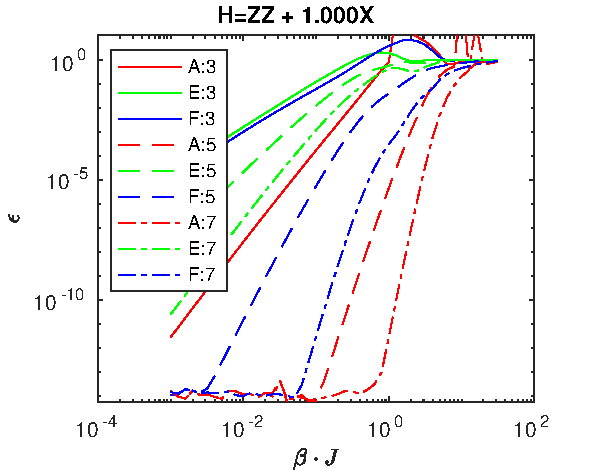
\includegraphics[height=0.9\textheight]{../Figuren/benchmarking/t_ising_small.pdf}
        \end{figure}
    \end{minipage}
    \begin{minipage}{.39\textwidth}

        \begin{itemize}
            \item Relative error $\epsilon$
            \item Different encodings:
                  \begin{itemize}
                      \item A: Small
                      \item E: Strict
                      \item F: well-conditioned
                  \end{itemize}

            \item bond dimension

                  \begin{table}[]
                      %\caption*{$\chi$}
                      \begin{tabular}{l l|l l }
                                                                 &   & \multicolumn{2}{c}{Encoding}       \\
                                                                 &   & A                            & E/F \\
                          \hline
                          \multirow{3}{*}{\rotatebox{90}{Order}} & 3 & 5                            & 10  \\
                                                                 & 5 & 21                           & 42  \\
                                                                 & 7 & 85                           & 170 \\
                      \end{tabular}
                  \end{table}

        \end{itemize}
    \end{minipage}

\end{frame}

\begin{frame}{Conclusion}
    \begin{itemize}
        \item Large $\beta$-steps
        \item Real time evolution
        \item Encoding
        \item Truncation $\chi$
    \end{itemize}
\end{frame}

\subsection{TFI Phase Diagram}

\begin{frame}{2D TFI: Introduction}
    \begin{minipage}{0.35\textwidth}
        \begin{itemize}
            \item Phase Transition
            \item Criticality
            \item Finite size scaling
                  \begin{itemize}
                      \item Observables:

                            $m$, $S$ and $\xi$
                      \item Parameters:

                            $T_c$, exponents
                  \end{itemize}
            \item $\Gamma=2.5$
            \item VUMPS ($\chi$,$\delta^{-1}$)
        \end{itemize}
    \end{minipage}
    \begin{minipage}{0.64\textwidth}
        \begin{figure}
            \centering
            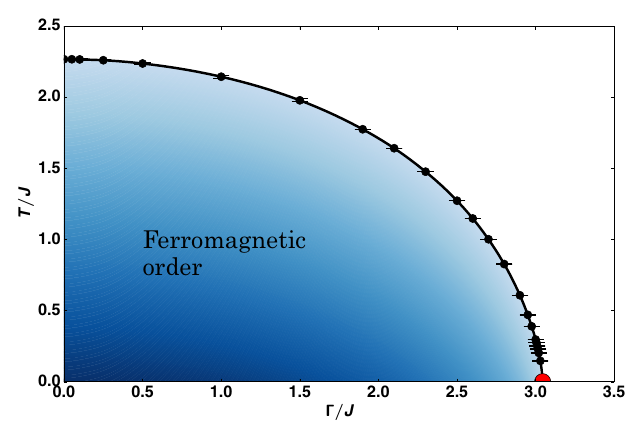
\includegraphics[width=\linewidth]{../Figuren/phsyics/2disingphase.png}
            \caption*{Figure taken from \cite{Hesselmann2016}  }
        \end{figure}
    \end{minipage}
\end{frame}

\begin{frame}{TFI Phase Diagram: $\Gamma=2.5$}
    \begin{minipage}{.75\textwidth}
        \begin{figure}
            \center
            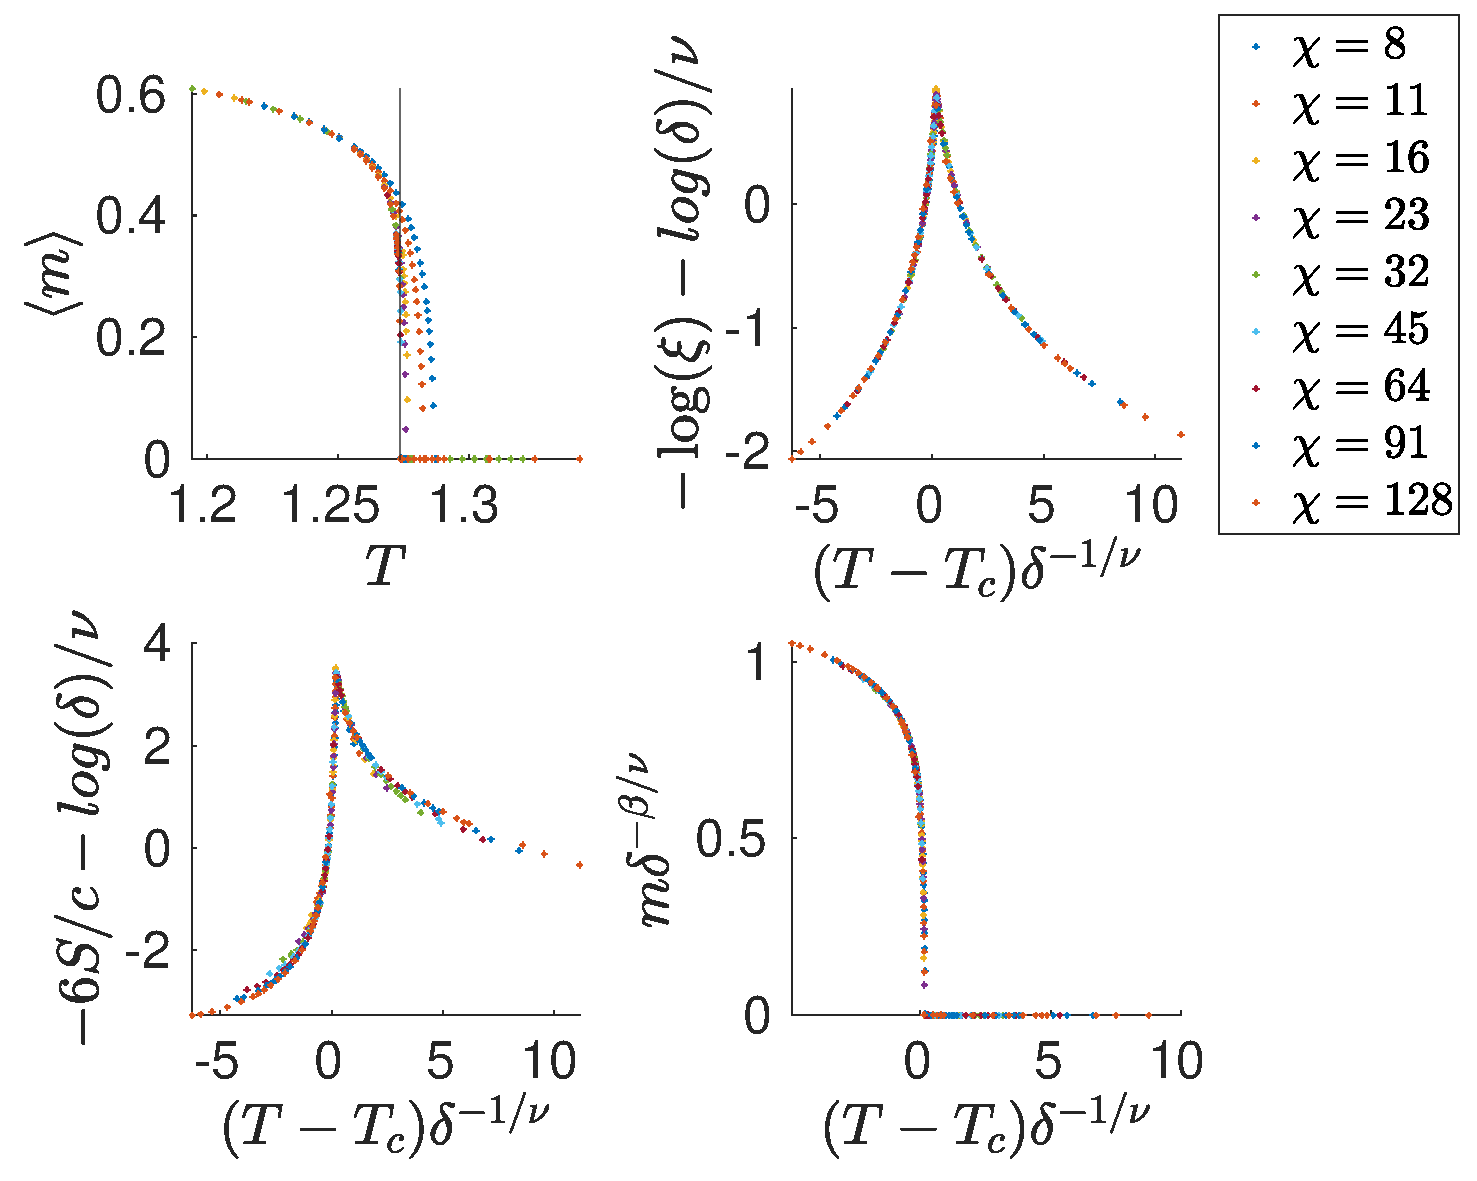
\includegraphics[height=\textheight]{../Figuren/phasediag/g25/zoomed_small.pdf}
        \end{figure}
    \end{minipage}
    \begin{minipage}{.24\textwidth}
        \begin{table}[]

            \begin{tabular}{l|l }
                    & $T_c$     \\
                \hline          \\
                Fit & 1.2736(6) \\
                QMC & 1.2737(6) \\
                TN  & 1.2737(2) \\
            \end{tabular}
            \caption*{Data from  \cite{Czarnik2019} }
        \end{table}
    \end{minipage}
\end{frame}



%5:20 min
%3:40

\section{Conclusion}
\begin{frame}{Conclusion}
    \begin{itemize}
        \item Cluster expansions work extremely well for some encodings
        \item Stable and fast framework
    \end{itemize}
\end{frame}

% \begin{frame}{Outlook}
%     \begin{itemize}
%         \item 3D
%         \item Incorperating internal symmetries
%         \item Lattices
%     \end{itemize}
% \end{frame}

%2 min

\begin{frame}[allowframebreaks]
    \frametitle{References}
    \bibliographystyle{elsarticle-num}
    \bibliography{../bib}
\end{frame}

\appendix
\backupbegin


\section{Tensor Networks}

\begin{frame}{Tensor Networks: Introduction}

    \begin{equation}
        \ket{\Psi} = \sum_{i_1 i_2 \cdots i_n } C^{i_1 i_2 \cdots i_n} \ket{i_1} \otimes \ket{i_2} \otimes \cdots \otimes \ket{i_n}.
    \end{equation}
    \begin{equation} \label{c_split}
        C^{i_1 i_2 \cdots i_n} = Tr( C^{i_1} C^{i_2} \cdots C^{i_n} M  ).
    \end{equation}

\end{frame}

\begin{frame}{Tensor Networks: Graphical Notation}
    \begin{table}[]
        \centering
        \begin{tabular}{l|l|l}
            conventional            & Einstein                & tensor notation           \\
            \hline
            $\Vec{x}$               & $x_{\alpha}$            &

            \begin{tikzpicture}[baseline=({N2.base}) ]
                \clip (-0.5,-0.5) rectangle (1,0.5);
                \node[circle, draw] (N2) at (0,0) {$x$};
                \node[] (N1) at (1,0) {};
                \draw  (N1) -- (N2) ;
            \end{tikzpicture}                                                     \\
            M                       & $M_{\alpha \beta}$      & \begin{tikzpicture}[baseline={0cm-0.5*height("$=$")} ]
                \clip (-1,-0.5) rectangle (1,0.5);

                \node[circle, draw] (N2) at (0,0) {$M$};
                \node[] (N0) at (-1,0) {};
                \node[] (N1) at (1,0) {};

                \draw  (N1) -- (N2) ;
                \draw  (N0) -- (N2) ;

            \end{tikzpicture} \\

            $\Vec{x} \cdot \Vec{y}$ & $x_{\alpha} y_{\alpha}$ & \begin{tikzpicture}[baseline=({N2.base}) ]
                \clip (-0.5,-0.5) rectangle (1.5,0.5);
                \node[circle, draw] (N2) at (0,0) {$x$};
                \node[circle, draw] (N1) at (1,0) {$y$};
                \draw  (N1) -- (N2) ;
            \end{tikzpicture} \\
        \end{tabular}
    \end{table}
\end{frame}

\begin{frame}{Tensor Networks: MPS}

    \begin{equation}
        C^{i_1 i_2 \cdots i_n} = Tr( C^{i_1} C^{i_2} \cdots C^{i_n} M )
    \end{equation}
    \begin{equation}
        \ctens  \; = \mpograph
    \end{equation}
\end{frame}

\begin{frame}{Tensor Networks: Operators}

    \begin{equation}
        \hat{O} =   \vcenter{\hbox{ \pepob{5}{3}{{
                            "-","-", "-","-",
                            "","","","",
                            "-","-", "-","-",}}{{
                            "-","-",
                            "","",
                            "","",
                            "","",
                            "-","-",}}{{
                            4,4,4,4,4,
                            13,0,0,0,13,
                            4,4,4,4,4,}} }}
    \end{equation}

    \begin{equation}
        \hat{O} \ket{\Psi} =  \vcenter{\hbox{ \pepob{5}{3}{{
                            "-","-", "-","-",
                            "","$\chi$","","",
                            "","$\chi$","","",}}{{
                            "-", "-",
                            "", "",
                            "", "",
                            "", "",
                            "-", "-",}}{{
                            4,4,4,4,4,
                            13,0,0,0,13,
                            13,0,0,0,13}}  }} =   \vcenter{\hbox{ \pepob{5}{2}{{
                            "-","-", "-","-",
                            "","$\chi^2$","",""}}{{
                            "-",
                            "",
                            "",
                            "",
                            "-"}}{{
                            4,4,4,4,4,
                            13,0,0,0,13}} }}
    \end{equation}

\end{frame}

\section{Linear Solver}

\begin{frame}{Linear Solver: Inversion Scheme}

    \begin{minipage}{0.4\textwidth}
        \only<1> { \begin{equation}
                \scalebox{0.9}{ \pepoat } \;  =  \; \scalebox{0.9}{\blockat}
            \end{equation}}
        \only<2-> {
            \begin{itemize}
                \only<2-> {\item Invert $A^i$ separately }
                      \only<2-3>{
                          \begin{itemize}
                              \item Fast
                              \item Numerically unstable
                          \end{itemize}
                      }
                      \only<4-> { \item Full inversion }
                      \only<4>{
                          \begin{itemize}
                              \item Slow
                              \item Stable for pseudoinverse
                          \end{itemize}
                      }
                      \only<5-> { \item Sparse full inversion }
                      \only<5>{
                          \begin{itemize}
                              \item $A^i = U^i \Sigma^i V^{i\dagger}$
                          \end{itemize}
                      }
            \end{itemize}
        }
    \end{minipage}
    \begin{minipage}{0.59\textwidth}
        \begin{equation}
            \only<1>  {  \vcenter{\hbox{   \scalebox{0.9}{  \pepoct }} } = \vcenter{\hbox{ \scalebox{0.9}{ \blockcta} }} }
            \only<2> { \vcenter{\hbox{  \scalebox{0.9}{  \pepocta } }}  =\vcenter{\hbox{ \scalebox{0.9}{  \blockcta }} }  }
            \only<3> { \vcenter{\hbox{ \scalebox{0.9}{  \pepoctb }}}  =\vcenter{\hbox{ \scalebox{0.9}{  \blockctb }} } }
            \only<4> { \vcenter{\hbox{ \scalebox{0.9}{  \pepoctc } }}  =\vcenter{\hbox{ \scalebox{0.9}{  \blockcta }} } }
            \only<5> { \vcenter{\hbox{\scalebox{0.9}{  \pepoctd }}}  =\vcenter{\hbox{ \scalebox{0.9}{  \blockcta }} } }
        \end{equation}
    \end{minipage}

\end{frame}

\section{Construction}

\begin{frame}{Notation}
    \begin{equation}
        O^{0 0} = \mpo{1}{ {0,0}  }{ {"$i$",}  }{ {"$j$",}}{}{{"",}} = \mpob{1}{ {0,0}  }{ {"$i$",}  }{ {"$j$",}}{}{{"",}}
    \end{equation}

    \begin{equation}
        O^{0 1} O^{1 0} = \mpob{2}{ {0,1,0}  }{ {"$i_1$","$i_2$"}  }{ {"$j_1$","$j_1$",}}{}{{"",}}
    \end{equation}

\end{frame}

\begin{frame}{General idea}
    \begin{equation}
        \mpob{1}{ {0,0}  }{}{}{}{{"",}} = \exp \left( -\beta H(\mpob{1}{}{}{}{}{{"",}})   \right)
    \end{equation}

    \begin{equation}
        \begin{split}
            \mpob{2}{ {0,1,0}  }{}{}{}{{"",}}  = \exp -\beta H( & \mpob{2}{ {,,} }{}{}{}{{"",}}) \\
            - &\mpob{2}{ {0,0,0}  }{}{}{}{{"",}}
        \end{split}
    \end{equation}

\end{frame}

\begin{frame}{General idea}
    \begin{equation}
        \begin{split}
            \only<1> { \mpob{3}{ {0,1,1,0}  }{}{}{}{{,,,}}  = \exp -\beta H( &   \mpob{3}{ {,,,} }{}{}{}{{,,}})  \\
                - \; &\mpob{3}{ {0,0,0,0}  }{}{}{}{{,,,}}\\
                - \;&\mpob{3}{ {0,1,0,0}  }{}{}{}{{,,,}}\\
                - \; &\mpob{3}{ {0,0,1,0}  }{}{}{}{{,,,}}}
            \only<2> {  \mpob{3}{ {0,1,1,0}  }{}{}{}{{,,,}}    = \exp -\beta H( &   \mpob{3}{ {,,,} }{}{}{}{{,,}})  \\[10pt]
                - \; &\mpob{3}{ {,,,}  }{}{}{}{{,,,}}}
            \only<3> {  \boxed{ \mpob{3}{ {0,1,1,0}  }{}{}{}{{,,,}} } }
        \end{split}
    \end{equation}
\end{frame}

\subsection{1D}
\begin{frame}{1D: Variant A}
    \begin{subequations}
        \begin{align}
             & \mpob{1}{ {,}  }{}{}{}{{,,}}                                      \\
             & \mpob{2}{ {,"1",}  }{}{}{}{{,,}}                                  \\
             & \mpob{3}{ {,"1","1",}  }{}{}{}{{,,,}}                             \\
             & \mpob{4}{ {,"1","2","1",}  }{}{}{}{{,,,,,}}    \label{2sitepatch} \\
             & \mpob{5}{ {,"1","2","2","1",}  }{}{}{}{{,,,,,}} \; .
        \end{align}
    \end{subequations}
\end{frame}

\begin{frame}{1D: Variant E}
    \begin{subequations}
        \begin{align}
             & \mpob{1}{ {,}  }{}{}{}{{,,}}                          \\
             & \mpob{2}{ {,"1",}  }{}{}{}{{,,}}                      \\
             & \mpob{3}{ {,"1","1'",}  }{}{}{}{{,,,}}                \\
             & \mpob{4}{ {,"1","2","1'",}  }{}{}{}{{,,,,,}}          \\
             & \mpob{5}{ {,"1","2","2'","1'",}  }{}{}{}{{,,,,,}} \;.
        \end{align}
    \end{subequations}
\end{frame}

\begin{frame}{1D: Variant F}
    \begin{subequations}
        \begin{align}
             & \mpob{1}{ {,}  }{}{}{}{{,,}}                                         \\
             & \mpob{2}{ {,"1'",}  }{}{}{}{{,,}}+  \mpob{2}{ {,"1",}  }{}{}{}{{,,}} \\
             & \mpob{3}{ {,"1","1",}  }{}{}{}{{,,,}}                                \\
             & \mpob{4}{ {,"1","2","1",}  }{}{}{}{{,,,,,}} \; +  \nonumber          \\
             & \mpob{4}{ {,"1","2'","1",}  }{}{}{}{{,,,,,}}                         \\
             & \mpob{5}{ {,"1","2","2","1",}  }{}{}{}{{,,,,,}} \;.
        \end{align}
    \end{subequations}
\end{frame}

\subsection{2D}

\begin{frame}
    \begin{equation}
        O^{0000} =  \vcenter{ \hbox{ \pepob{4}{3}{{
                            "-","-","-",
                            "-","0","0",
                            "-","-","-"}}{{
                            "-","-",
                            "-","-",
                            "0","0",
                            "-","-"}}{{
                            1,1,4,1,
                            1,4,12,4,
                            1,1,4,1}} }} = \mpob{1}{ {,}  }{}{}{}{{,,}}
    \end{equation}
\end{frame}

\begin{frame}{2D: Linear Blocks}
    \begin{subequations}
        \begin{align}
             & \vcenter{\hbox{ \pepob{2}{2}{{"1",,}}{{,,}}{{0,0,1,1}} }}                                                                                                                                   \\[0.5cm]
             & \vcenter{\hbox{  \pepob{2}{2}{{"1","1",}}{{"1","1",}}{{0,0,0,1}} }}\;
            \vcenter{\hbox{  \pepob{3}{2}{{"1","1","1","1"}}{{"1","1","1","1"}}{{0,0,0,1,1,1}} }}                                                                                                          \\[0.5cm]
             & \vcenter{\hbox{  \pepob{3}{2}{{"1","1","1","1"}}{{"1","1","1","1"}}{{0,0,0,1,0,1}} \quad   \pepob{3}{3}{{"1","1","1","1","1","1",}}{{"1","1","1","1","1","1",}}{{1,0,1,0,0,0,1,0,1}}  }} \;
        \end{align}
    \end{subequations}
\end{frame}

\begin{frame}{2D: Nonlinear Blocks}
    \begin{equation}
        \vcenter{\hbox{   {\pepob{2}{2}{{"$\alpha$","$\alpha$",}}{{"$\alpha$","$\alpha$",}}{{0,0,0,0}}} }}
    \end{equation}

    \begin{equation}
        \vcenter{\hbox{     \pepob{5}{3}{{
                            "-","-", "-",     "-",
                            "-","1","$\beta$","-",
                            "-","-","$\alpha$","-"}}{{
                            "-","-",
                            "-","-",
                            "-","$\gamma$",
                            "-","$\alpha$",
                            "-","-"}}{{
                            1,1,1,1,1,
                            1,0,0,0,1,
                            1,1,0,0,1}} }} \; .
    \end{equation}
\end{frame}

\section{$\Gamma = 2.9$}

\begin{frame}
    \begin{figure}
        \center
        \includegraphics[height=\textheight]{../Figuren/phasediag/g29/a.pdf}
    \end{figure}
\end{frame}

\section{Solvers}
\subsection{Linear Solver}

\def \pepoat {\begin{tikzpicture}[baseline=0.5]

        \def \legLength { 0.8}
        \def \radius {0.1}

        \pgfmathsetmacro{\step}{2*\radius+ \legLength} % 1
        \pgfmathsetmacro{\legpos}{\radius+\legLength} %0.9

        \node[draw,minimum size=0.6cm] (O0) at (0,0) {X};
        \draw (0.15,0.15) -- ++(0.3,0.3);

        \node[draw, circle,radius=\radius] (L1) at (-1,0) {};
        \node[draw, circle,radius=\radius] (L2) at (-2,0) {};
        \node[draw, circle,radius=\radius] (L3) at (-3,0) {};

        \node[draw, circle,radius=\radius] (U1) at (0,1) {};
        \node[draw, circle,radius=\radius] (U2) at (0,2) {};

        \node[draw, circle,radius=\radius] (D1) at (0,-1) {};

        \node[draw, circle,radius=\radius] (R1) at (1,0) {};

        \draw (O0) -- node [above] {3}  (L1);
        \draw (L2) -- node [above] {2}  (L1);
        \draw (L2) -- node [above] {1}  (L3);

        \draw (O0) -- node [left] {2}  (U1);
        \draw (U2) -- node [left] {1}  (U1);

        \draw (O0) -- node [above] {1}  (R1);

        \draw (O0) --  node [left] {1} (D1);

        \draw (L1.center) -- ++(0.2,0.2);
        \draw (L2.center) -- ++(0.2,0.2);
        \draw (L3.center) -- ++(0.2,0.2);
        \draw (U1.center) -- ++(0.2,0.2);
        \draw (U2.center) -- ++(0.2,0.2);
        \draw (R1.center) -- ++(0.2,0.2);
        \draw (D1.center) -- ++(0.2,0.2);

    \end{tikzpicture}}

\def \blockat {  \begin{tikzpicture}[baseline=0.5]

        \def \legLength { 0.8}
        \def \radius {0.1}

        \pgfmathsetmacro{\step}{2*\radius+ \legLength} % 1
        \pgfmathsetmacro{\legpos}{\radius+\legLength} %0.9

        %\node[draw=none] (O0) at (0,0) {};
        \node[draw=none,minimum size=0.6cm] (O0) at (0,0) {B};
        \draw (0.15,0.15) -- ++(0.3,0.3);

        \node[draw=none] (L1) at (-1,0) {};
        \node[draw=none] (L2) at (-2,0) {};
        \node[draw=none] (L3) at (-3,0) {};

        \node[draw=none] (U1) at (0,1) {};
        \node[draw=none] (U2) at (0,2) {};

        \node[draw=none] (D1) at (0,-1) {};

        \node[draw=none] (R1) at (1,0) {};

        %\draw (O0.center) -- ++(0.45,0.45);
        \draw (L1.center) -- ++(0.2,0.2);
        \draw (L2.center) -- ++(0.2,0.2);
        \draw (L3.center) -- ++(0.2,0.2);
        \draw (U1.center) -- ++(0.2,0.2);
        \draw (U2.center) -- ++(0.2,0.2);
        \draw (R1.center) -- ++(0.2,0.2);
        \draw (D1.center) -- ++(0.2,0.2);

        \draw (-3.3,0.3)--(-0.3,0.3) -- (-0.3,2.3)--(0.3,2.3)
        -- (0.3,0.3) -- (1.3,0.3) -- (1.3,-0.3) -- (0.3,-0.3)
        -- (0.3,-1.3) -- (-0.3, -1.3) -- (-0.3,-0.3) -- (-3.3,-0.3) -- cycle;

    \end{tikzpicture}}

\def \pepobt {\begin{tikzpicture}[baseline=0.5]

        \def \legLength { 0.8}
        \def \radius {0.1}

        \pgfmathsetmacro{\step}{2*\radius+ \legLength} % 1
        \pgfmathsetmacro{\legpos}{\radius+\legLength} %0.9

        %\node[draw, circle, radius=\radius] (O0) at (0,0) {};
        \node[draw,minimum size=0.6cm] (O0) at (0,0) {X};
        \draw (0.15,0.15) -- ++(0.3,0.3);

        \node[draw, minimum size=0.6cm] (L1) at (-1,0) {};
        \node[draw, minimum size=0.6cm] (U1) at (0,1) {};
        \node[draw, minimum size=0.6cm] (D1) at (0,-1) {};
        \node[draw, minimum size=0.6cm] (R1) at (1,0) {};

        \draw (O0) -- (L1);
        \draw (O0) -- (U1);
        \draw (O0) -- (R1);
        \draw (O0) -- (D1);

        %\draw(O0.center) -- ++(0.2,0.2);
        \draw[line width=0.75mm]  (L1.center) -- ++(0.2,0.2);
        \draw[line width=0.75mm] (U1.center) -- ++(0.2,0.2);
        \draw[line width=0.75mm] (R1.center) -- ++(0.2,0.2);
        \draw[line width=0.75mm] (D1.center) -- ++(0.2,0.2);

    \end{tikzpicture} }

\def \blockbt {   \begin{tikzpicture}[baseline=0.5]

        \def \legLength { 0.8}
        \def \radius {0.1}

        \pgfmathsetmacro{\step}{2*\radius+ \legLength} % 1
        \pgfmathsetmacro{\legpos}{\radius+\legLength} %0.9

        %\node[draw=none] (O0) at (0,0) {};
        \node[draw=none,minimum size=0.6cm] (O0) at (0,0) {B};
        \draw (0.15,0.15) -- ++(0.3,0.3);

        \node[draw=none] (L1) at (-1,0) {};
        \node[draw=none] (L2) at (-2,0) {};
        \node[draw=none] (L3) at (-3,0) {};

        \node[draw=none] (U1) at (0,1) {};
        \node[draw=none] (U2) at (0,2) {};

        \node[draw=none] (D1) at (0,-1) {};

        \node[draw=none] (R1) at (1,0) {};

        %\draw (O0.center) -- ++(0.45,0.45);
        \draw[line width=0.75mm] (L3.center) -- ++(0.2,0.2);
        \draw[line width=0.75mm] (U2.center) -- ++(0.2,0.2);
        \draw[line width=0.75mm] (R1.center) -- ++(0.2,0.2);
        \draw[line width=0.75mm] (D1.center) -- ++(0.2,0.2);

        \draw (-3.3,0.3)--(-0.3,0.3) -- (-0.3,2.3)--(0.3,2.3)
        -- (0.3,0.3) -- (1.3,0.3) -- (1.3,-0.3) -- (0.3,-0.3)
        -- (0.3,-1.3) -- (-0.3, -1.3) -- (-0.3,-0.3) -- (-3.3,-0.3) -- cycle;

    \end{tikzpicture} }

\def \pepoct { \begin{tikzpicture}[baseline=0.5]
        \draw (0,2.5)-- (0,-1.5) -- (1,-1.5)-- (1,2.5) -- cycle;

        \node[draw=none] (x)  at (0.5,0.5) {X};

        \node[draw, minimum size=0.6cm] (n1)  at (-1,2) {$A^1$};
        \node[draw, minimum size=0.6cm] (n2)  at (-1,1) {$A^2$};
        \node[draw, minimum size=0.6cm] (n3)  at (-1,0) {$A^3$};
        \node[draw, minimum size=0.6cm] (n4)  at (-1,-1) {$A^4$};

        \draw (n1) -- node [above] {$\alpha_1$} (0,2);
        \draw (n2) -- node [above] {$\alpha_2$} (0,1);
        \draw (n3) -- node [above] {$\alpha_3$} (0,0);
        \draw (n4) -- node [above] {$\alpha_4$} (0,-1);

        \draw[line width=0.75mm] (n1) -- ++(-0.6,0) node [left] {$I^1$};
        \draw[line width=0.75mm] (n2) -- ++(-0.6,0) node [left] {$I^2$};
        \draw[line width=0.75mm] (n3) -- ++(-0.6,0) node [left] {$I^3$};
        \draw[line width=0.75mm] (n4) -- ++(-0.6,0) node [left] {$I^4$};

        \draw (1,0.5) -- (1.3,0.5)  node [right] {$j$} ;

    \end{tikzpicture} }

\def \blockct { \begin{tikzpicture}[baseline=3]
        \draw (0,2.5)-- (0,-1.5) -- (1,-1.5)-- (1,2.5) -- cycle;

        \node[draw=none] (x)  at (0.5,0.5) {B};

        \draw[line width=0.75mm] (-0.3,2)  node [left] {$I^1$}  -- (0,2) ;
        \draw[line width=0.75mm] (-0.3,1)  node [left] {$I^2$} -- (0,1);
        \draw[line width=0.75mm] (-0.3,0)  node [left] {$I^3$} -- (0,0);
        \draw[line width=0.75mm] (-0.3,-1)  node [left] {$I^4$} -- (0,-1);

        \draw (1,0.5) -- (1.3,0.5)  node [right] {$j$} ;

    \end{tikzpicture} }

\begin{frame}{Linear Solver: Standard Form}
    \begin{equation}
        \only<1>{ \vcenter{\hbox{ \pepob{5}{5}{{
                                "-","-","-","-",
                                "-","-","-","-",
                                "1","2","3","1",
                                "-","-","-","-",
                                "-","-","-","-"}}{{
                                "-","-","-","-",
                                "-","-","-","-",
                                "-","-","-","-",
                                "-","1","2","1",
                                "-","-","-","-"}}{{
                                1,1,1,1,1,
                                1,1,1,0,1,
                                0,0,0,0,0,
                                1,1,1,0,1,
                                1,1,1,0,1}} }} }
        \only<2>{  \pepoat \;  =  \;\blockat  }
        \only<3>{ \pepobt \;  =  \;\blockbt }
        \only<4>{ \vcenter{\hbox{ \pepoct }}  =\vcenter{\hbox{  \blockct }} }
    \end{equation}
\end{frame}

\begin{frame}{Linear Solver: Inversion Scheme}
    \begin{itemize}
        \only<1-> {\item Invert $A^i$ separately }
              \only<1>{
                  \begin{itemize}
                      \item Fast
                      \item Numerically unstable
                  \end{itemize}
              }
              \only<2-> { \item Full inversion $A = A^1 \otimes A^2 \cdots \otimes A^m$ }
              \only<2>{
                  \begin{itemize}
                      \item Slow
                      \item Stable for pseudoinverse
                  \end{itemize}
              }
              \only<3-> { \item Sparse full inversion }
              \only<3>{
                  \begin{itemize}
                      \item $A^i = U \Sigma V^{\dagger}$
                      \item $S = S^1 \otimes S^2 \cdots \otimes S^m$
                  \end{itemize}
              }
    \end{itemize}

\end{frame}

\begin{frame}{Linear Solver: Applicability}
    \begin{equation}
        \vcenter{\hbox{  \begin{tikzpicture}[baseline=0.5]

                    \def \legLength { 0.8}
                    \def \radius {0.1}

                    \pgfmathsetmacro{\step}{2*\radius+ \legLength} % 1
                    \pgfmathsetmacro{\legpos}{\radius+\legLength} %0.9

                    \node[draw, circle,radius=\radius] (L0) at (-1,0) {};

                    \draw (-0.3,0.3) -- (0.3,0.3) -- (0.3,-0.3) -- (-0.3,-0.3) -- cycle;

                    \node[draw, circle,radius=\radius] (R0) at (1,0) {};
                    \node[draw, circle,radius=\radius] (R1) at (1,1) {};

                    \node[draw, circle,radius=\radius] (U) at (0,1) {};
                    \node[draw, circle,radius=\radius] (D) at (0,-1) {};

                    \draw (R0) --   (R1);

                    \draw (L0) --   (-0.3,0);

                    \draw (R0) --   (0.3,0);
                    \draw (U) --   (0,0.3);
                    \draw (D) --   (0,-0.3);
                    \draw (R1) --   (U);

                    \node[draw=none] (C0) at (0,0) {X};
                \end{tikzpicture} }}
    \end{equation}
\end{frame}

\def \figa { \vcenter{\hbox{ \pepob{5}{3}{{
                        "","","","",
                        "","","","",
                        "","","",""}}{{
                        "","",
                        "","",
                        "","",
                        "","",
                        "",""}}{{
                        1,1,1,1,1,
                        1,0,0,0,1,
                        1,0,0,0,1}} } }}

\def \figb { \vcenter{\hbox{  \begin{tikzpicture}[baseline=0.5]

                \def \legLength { 0.8}
                \def \radius {0.1}

                \pgfmathsetmacro{\step}{2*\radius+ \legLength} % 1
                \pgfmathsetmacro{\legpos}{\radius+\legLength} %0.9

                \node[draw, circle,radius=\radius] (L0) at (-1,0) {};
                \node[draw, circle,radius=\radius] (L1) at (-1,1) {};

                \draw (-0.3,1.3) -- (0.3,1.3) -- (0.3,-0.3) -- (-0.3,-0.3) -- cycle;

                \node[draw, circle,radius=\radius] (R0) at (1,0) {};
                \node[draw, circle,radius=\radius] (R1) at (1,1) {};

                \draw (L0) --   (L1);
                \draw (R0) --   (R1);

                \draw (L0) --   (-0.3,0);
                \draw (L1) --   (-0.3,1);

                \draw (R0) --   (0.3,0);
                \draw (R1) --   (0.3,1);

                \node[draw=none] (C0) at (0,0.5) {X};
            \end{tikzpicture}}}}

\def \figc {\vcenter{\hbox{  \begin{tikzpicture}[baseline=0.5]

                \def \legLength { 0.8}
                \def \radius {0.1}

                \pgfmathsetmacro{\step}{2*\radius+ \legLength} % 1
                \pgfmathsetmacro{\legpos}{\radius+\legLength} %0.9

                \node[draw=none, circle,radius=\radius] (L0) at (-1,0) {};
                \node[draw=none, circle,radius=\radius] (L1) at (-1,1) {};

                \draw (-0.3,1.3) -- (0.3,1.3) -- (0.3,-0.3) -- (-0.3,-0.3) -- cycle;

                \node[draw=none, circle,radius=\radius] (R0) at (1,0) {};
                \node[draw=none, circle,radius=\radius] (R1) at (1,1) {};

                \draw (L0) --   (-0.3,0);
                \draw (L1) --   (-0.3,1);

                \draw (R0) --   (0.3,0);
                \draw (R1) --   (0.3,1);

                \node[draw=none] (C0) at (0,0.5) {X};
            \end{tikzpicture} }} }

\def \figd {\vcenter{\hbox{  \begin{tikzpicture}[baseline=0.5]

                \def \legLength { 0.8}
                \def \radius {0.1}

                \pgfmathsetmacro{\step}{2*\radius+ \legLength} % 1
                \pgfmathsetmacro{\legpos}{\radius+\legLength} %0.9

                \node[draw=none, circle,radius=\radius] (L0) at (-1,0) {};
                \node[draw=none, circle,radius=\radius] (L1) at (-1,1) {};

                \node[draw, circle,radius=\radius] (C0) at (0,0) {};
                \node[draw, circle,radius=\radius] (C1) at (0,1) {};

                \node[draw=none, circle,radius=\radius] (R0) at (1,0) {};
                \node[draw=none, circle,radius=\radius] (R1) at (1,1) {};

                \draw (L0) --   (C0);
                \draw (L1) --   (C1);

                \draw (R0) --   (C0);
                \draw (R1) --   (C1);

                \draw (C1) --   (C0);
            \end{tikzpicture} }}}

\begin{frame}{Linear Solver: Applicability}
    \begin{equation}
        \figa
    \end{equation}

    \begin{subequations}
        \begin{align}
             & \figb          \\
             & \figc =  \figd
        \end{align}
    \end{subequations}
\end{frame}

\subsection{Nonlinear Solver}
\begin{frame}{Nonlinear Solver}
    \begin{itemize}
        \item Nonlinear least squares
        \item Jacobian
        \item Permutations
    \end{itemize}
\end{frame}

\subsection{Sequential Linear Solver}
\begin{frame}{Sequential Linear Solver}
    \begin{itemize}
        \item Based on linear solver
        \item Sweep over unknown tensors
        \item Permutations
    \end{itemize}
\end{frame}

\backupend

\end{document}